%\chapter[Guaranteed Consensus of Double-Integrator Systems in the Presence of Directed Cycles]{Guaranteed Consensus of Double-Integrator Systems in the Presence of Directed Cycles\footnote{The core theoretical algorithms and formulations in this chapter are derived in part from the author's published work in the \emph{Proceedings of the American Control Conference (ACC)}. This chapter expands upon those preliminary manuscripts by providing unified proofs, comprehensive sub-block matrix extensions, and root-locus design frameworks.}}\label{ch:Guaranteed_Consensus}
\chapter[Guaranteed Consensus in Directed Cyclic Networks]{Guranteed Consensus of Double-Integrators in the Presence of Directed Cycles\footnote{The theoretical formulations of the problems and the algorithms have some overlap with the author's published work in the \emph{Proceedings of the American Control Conference (ACC) 2023}. This chapter expands upon the preliminary results by providing detailed proofs, comprehensive sub-block matrix extensions, and root-locus based design frameworks.}}\label{ch:Guaranteed_Consensus}

\section{Introduction}\label{sec:ch_GC_intro_Guaranteed_Consensus}
As established in Chapters \ref{ch:intro} and \ref{ch:TwoReverseEdges}, second-order consensus over directed graphs exhibits a fundamental vulnerability: the introduction of reverse feedback channels forms directed cycles. These cycles introduce complex-conjugate eigenvalues into the graph Laplacian spectrum $\sigma(\mathcal{L})$, inducing phase lag between position alignment and velocity damping. As proven by Ren and Atkins \cite{ren2005second} and Yu et al. \cite{yu2010some}, second-order consensus breaks down completely unless the velocity coupling parameter $\gamma$ exceeds a critical lower threshold dictated by the Laplacian spectrum:
\begin{equation}\label{eq:ch_GC_yu_threshold_recap}
    \gamma > \max_{i \in \{2, \dots, N\}} \frac{|\mathfrak{Im}(\lambda_i)|}{|\lambda_i|} \sqrt{\frac{1}{\mathfrak{Re}(\lambda_i)}}
\end{equation}
In practical hierarchical networks— such as organizational swarms, industrial automated guided vehicles (AGVs), or multi-tiered power grids— reverse communication links frequently arise due to localized feedback, spatial proximity, or status reporting. When a reverse edge is added to an operational network with a predesigned, fixed coupling parameter $\gamma$, condition \eqref{eq:ch_GC_yu_threshold_recap} is easily violated, leading to severe dynamic instability.
\begin{figure}[ht!]
	\centering
	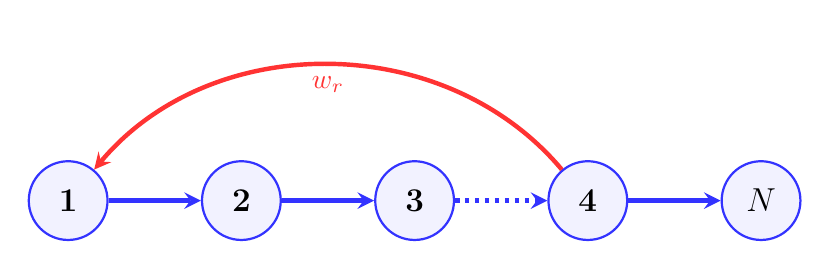
\begin{tikzpicture}[node distance=2.2cm, state/.style={circle, draw=blue!80, fill=blue!5, thick, minimum size=1.0cm, font=\large\bfseries}]
		\node[state] (1) {1};
		\node[state] (2) [right of=1] {2};
		\node[state] (3) [right of=2] {3};
		\node[state] (4) [right of=3] {4};
		\node[state] (5) [right of=4] {$N$};
		
		\path [->, >=stealth, ultra thick, blue!80] (1) edge (2);
		\path [->, >=stealth, ultra thick, blue!80] (2) edge (3);
		\path [->, >=stealth, ultra thick, blue!80] (3) edge[dotted] (4);
		\path [->, >=stealth, ultra thick, blue!80] (4) edge (5);
		\path [->, >=stealth, ultra thick, red!80] (4) edge[bend right=50] node[below] {$w_r$} (1);
	\end{tikzpicture}
	\caption{Directed chain network with a reverse feedback edge entering the leader node ($x_1 = 1$), forming a root-node loop.}
	\label{fig:LeaderCycleNetwork}
\end{figure}
\begin{figure}[ht!]
	\centering
	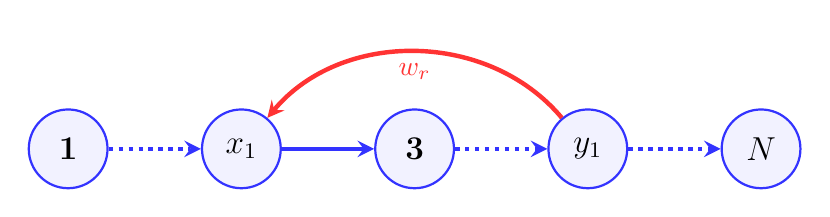
\begin{tikzpicture}[node distance=2.2cm, state/.style={circle, draw=blue!80, fill=blue!5, thick, minimum size=1.0cm, font=\large\bfseries}]
		\node[state] (1) {1};
		\node[state] (2) [right of=1] {$x_1$};
		\node[state] (3) [right of=2] {3};
		\node[state] (4) [right of=3] {$y_1$};
		\node[state] (5) [right of=4] {$N$};
		
		\path [->, >=stealth, ultra thick, blue!80] (1) edge[dotted] (2);
		\path [->, >=stealth, ultra thick, blue!80] (2) edge (3);
		\path [->, >=stealth, ultra thick, blue!80] (3) edge[dotted] (4);
		\path [->, >=stealth, ultra thick, blue!80] (4) edge[dotted] (5);
		\path [->, >=stealth, ultra thick, red!80] (4) edge[bend right=50] node[below] {$w_r$} (2);
	\end{tikzpicture}
	\caption{Directed chain network with a reverse feedback edge strictly exterior to the leader node ($x_1 > 1$).}
	\label{fig:LeaderlessCycleNetwork}
\end{figure}
In Chapter \ref{ch:TwoReverseEdges}, we established two major analytical barriers to mitigating this breakdown:
\begin{itemize}
    \item \textbf{High Computational and Communication Overhead of Global Retuning:} Restoring stability by adjusting $\gamma$ globally requires every agent in the network to access the updated global Laplacian spectrum $\sigma(\mathcal{L})$, destroying the decentralized nature of the network protocol.
    \item \textbf{The Root-Node Loop Structural Singularity:} When a reverse edge enters the root/leader node itself ($x_1 = 1$, as shown in Figure \ref{fig:LeaderCycleNetwork}), standard characteristic polynomial methods collapse ($s_1 = 1 \implies \lambda_2 = 0$). The leader node loses its zero in-degree property ($d_{\text{in}, 1} > 0$), destroying the leader-follower hierarchy and converting every node in the loop into an equivalent root node.
\end{itemize}

\subsection*{Summary of Chapter Contributions}
To resolve these challenges, this chapter synthesizes a suite of \textbf{fully localized control remedies} that guarantee second-order consensus under fixed global coupling parameters $\gamma$. The specific contributions are:
\begin{enumerate}
    \item \textbf{Decentralized Gershgorin--Based Perturbation Framework (Leader -- Exterior Loops):} For directed cycles that do not contain the leader/root node ($x_1 > 1$, Figure \ref{fig:LeaderlessCycleNetwork}), we formulate \textbf{Node-Scaling, Edge-Scaling, and Combined-Scaling} algorithms. By constructing optimal Arithmetic Progressions (AP) of Gershgorin column discs, we guarantee that the minimum real eigenvalue component satisfies $\mathfrak{Re}(\lambda_2) \ge 1/\gamma^2$, ensuring consensus through localized gains confined strictly to loop agents and edges.
    \item \textbf{Resolution of the Root-Node Loop Singularity via Complementary Root-Locus:} For directed cycles that incorporate the leader node ($x_1 = 1$, Figure \ref{fig:LeaderCycleNetwork}), where Gershgorin-based methods fail, we formulate a complementary root-locus control framework. By modeling loop gain shifts via $G(s) = \frac{\beta\{(s-\alpha)^\ell - (-\alpha)^\ell\}}{s(s-\alpha)^\ell}$, we derive precise gain bounds on $\alpha$ and $\beta$ that guarantee stability.
    \item \textbf{Equal-Weight Cyclic Pursuit Synthesis:} To prevent edge-weakening under root-node loops, we derive an exact closed-form single-gain threshold ($\alpha \ge \frac{\cot^2(\pi/(\ell+1))}{2\gamma^2}$) based on cyclic pursuit, guaranteeing consensus while maintaining equal edge weights across all agents in the directed cycle.
\end{enumerate}
\section{Mathematical Preliminaries and Problem Formulation} \label{sec:ch_GC_prelims}
This section formalizes the network state equations, graph-theoretic structures, and fundamental mathematical lemmas required to develop localized perturbation remedies.
\subsection{System Dynamics and Laplacian Matrix Partitions}
Consider an $N$-agent multi-agent system interacting over a directed graph $\mathcal{G} = (\mathcal{V}_g, \mathcal{E}_g, \mathcal{W}_g)$. Recall from Section \ref{sec:ch_TRE_Prelims} that the translational motion of agent $i \in \{1, 2, \dots, N\}$ in $d$-dimensional space is governed by double-integrator dynamics $\dot{p}_i = v_i, \dot{v}_i = u_i$. Under the local control protocol \eqref{eq:ch_TRE_agent_wise}:
\begin{equation} \label{eq:ch_GC_control_law}
	u_i(t) = -\sum_{j=1}^{N} w_{ij} \left[ (p_i(t) - p_j(t)) + \gamma (v_i(t) - v_j(t)) \right], \quad i \in \{1, 2, \dots, N\}
\end{equation}
where $w_{ij}$ is the $(i,j)$-th entry of the weighted adjacency matrix $\mathcal{W}_g$, and $\gamma > 0$ is the predesigned, fixed global velocity coupling parameter. Stacking composite states into $\mathcal{X}(t) \coloneqq [p^T(t), v^T(t)]^T \in \mathbb{R}^{2Nd}$, the global system evolves according to $\dot{\mathcal{X}}(t) = (\hat{\mathcal{L}} \otimes I_d) \mathcal{X}(t)$, where:
\begin{equation}\label{eq:ch_GC_hat_laplacian}
	\hat{\mathcal{L}} = \begin{bmatrix} 0_{N \times N} & I_N \\ -\mathcal{L} & -\gamma \mathcal{L} \end{bmatrix} \in \mathbb{R}^{2N \times 2N}
\end{equation}

When the interaction graph is a nominal $N$-node directed chain indexed by topological ordering (Definition \ref{def:ch_TRE_chaindigraph}), the graph Laplacian $\mathcal{L}$ is strictly lower triangular. When a reverse edge of weight $w_r > 0$ is inserted from tail node $y_1$ to head node $x_1$ ($y_1 > x_1$), forming a cycle of range $\ell = y_1 - x_1$, the structure of $\mathcal{L}$ depends on whether the leader node ($x_1 = 1$) is involved:

1. Leader-Exterior Loop ($x_1 > 1$, Figure \ref{fig:LeaderlessCycleNetwork}):
   \begin{equation} \label{eq:ch_GC_OriginalLaplacian}
   	\mathcal{L}_{\text{ext}} = \begin{bmatrix}
   		\mathcal{L}_1 & 0 & 0 \\
   		* & \mathcal{C} + \mathcal{L}_{\text{re}} & 0 \\
   		* & * & \mathcal{L}_2
   	\end{bmatrix}
   \end{equation}
   where $\mathcal{L}_1 \in \mathbb{R}^{(x_1-1) \times (x_1-1)}$ and $\mathcal{L}_2 \in \mathbb{R}^{(N-y_1) \times (N-y_1)}$ are lower triangular sub-matrices corresponding to unperturbed chain segments, $\mathcal{C} \in \mathbb{R}^{(\ell+1) \times (\ell+1)}$ represents the nominal sub-chain, and $\mathcal{L}_{\text{re}}$ captures the additive perturbation due to the reverse edge:
   \begin{equation}\label{eq:ch_GC_ReverseEdgeMatrix}
   	\mathcal{L}_{\text{re}} = \begin{bmatrix}
   		w_r & 0 & \dots & 0 & -w_r \\
   		0 & 0 & \dots & 0 & 0 \\
   		\vdots & \vdots & \ddots & \vdots & \vdots \\
   		0 & 0 & \dots & 0 & 0
   	\end{bmatrix} \in \mathbb{R}^{(\ell+1) \times (\ell+1)}
   \end{equation}

2. Root-Node Loop ($x_1 = 1$, Figure \ref{fig:LeaderCycleNetwork}):
   \begin{equation} \label{eq:ch_GC_OriginalLaplacianleader}
   	\mathcal{L}_{\text{root}} = \begin{bmatrix}
   		\mathcal{C} + \mathcal{L}_{\text{re}} & 0 \\
   		* & \mathcal{L}_2
   	\end{bmatrix}
   \end{equation}
   where $\mathcal{C} + \mathcal{L}_{\text{re}} \in \mathbb{R}^{(\ell+1) \times (\ell+1)}$ is a circulant-like block containing the zero eigenvalue $\lambda_1 = 0$.

Because of the block lower-triangular structure in \eqref{eq:ch_GC_OriginalLaplacian} and \eqref{eq:ch_GC_OriginalLaplacianleader}, the non-zero complex spectrum of $\mathcal{L}$ is determined entirely by the sub-block $\mathcal{C} + \mathcal{L}_{\text{re}}$.

\subsection{Foundational Stability Criteria and Problem Statement}

Recall from Lemma \ref{lem:ch_TRE_sufficiencyren} and Equation \eqref{eq:ch_TRE_DubeyBound} that second-order consensus is guaranteed if the non-zero Laplacian spectrum satisfies:
\begin{equation}\label{eq:ch_GC_dubey_bound}
    \mathfrak{Re}(\lambda_i) \ge \mathfrak{Re}(\lambda_2) \ge \frac{1}{\gamma^2}, \quad \forall i \in \{2, \dots, N\}
\end{equation}
Condition \eqref{eq:ch_GC_dubey_bound} provides a clear goal to be met: to guarantee consensus under a fixed global coupling gain $\gamma$, local control gain readjustments must shift the spectrum of $\mathcal{C} + \mathcal{L}_{\text{re}}$ so that every non-zero eigenvalue resides to the right of the vertical line $\mathfrak{Re}(z) = 1/\gamma^2$ in the complex plane.

This immediately leads to the core problem addressed in this chapter.

\begin{problem}\label{prob:ch_GC_main_problem}
Consider an $N$-node directed chain of double-integrator agents operating under protocol \eqref{eq:ch_GC_control_law} with a fixed, predesigned velocity coupling parameter $\gamma > 0$. Suppose a reverse feedback edge is added, forming a directed cycle of range $\ell \coloneqq y_1 - x_1$. Synthesize localized node/edge parameter tuning strategies confined strictly to the agents and edges participating in (or adjacent to) the cycle such that second-order consensus is guaranteed without adjusting global parameters ($\gamma$) or requiring all the agents to access the global Laplacian spectrum $\sigma(\mathcal{L})$.
\end{problem}

\subsection{Mathematical Toolset}
To resolve Problem \ref{prob:ch_GC_main_problem}, we utilize Gershgorin's Disc Theorem along with three key algebraic/geometric propositions.
\begin{theo}[Gershgorin's Disc Theorem \cite{horn2012matrix}]\label{thm:ch_GC_GershgorinDiscTheorem}
Let $A = [a_{ij}] \in \mathbb{R}^{n \times n}$ be a square matrix. For each column $j \in \{1, 2, \dots, n\}$, define the deleted column-sum radius $R_j(A) \coloneqq \sum_{i=1, i \neq j}^{n} |a_{ij}|$. Associated with column $j$, define the closed Gershgorin disc $\mathfrak{D}_j(A)$ in the complex plane $\mathbb{C}$:
\begin{equation}
	\mathfrak{D}_j(A) \coloneqq \left\{ z \in \mathbb{C} : |z - a_{jj}| \le R_j(A) \right\}
\end{equation}
All eigenvalues $\lambda \in \sigma(A)$ lie within the union of these $n$ column discs: $\sigma(A) \subset \bigcup_{j=1}^{n} \mathfrak{D}_j(A)$. By matrix transposition ($\sigma(A) = \sigma(A^T)$), identical statements hold for row-sum radii.
\end{theo}
\begin{proposition}[Polynomial Root Reflection]\label{prop:ch_GC_polynomialreflection}
If $f(x) = \sum_{i=0}^{n} a_i x^i$ is a polynomial with real coefficients $a_i \in \mathbb{R}$ having roots $x_i \in \mathbb{C}$, then the polynomial $f(-x)$ has roots given by $-x_i^*$, where $(\cdot)^*$ denotes complex conjugation.
\end{proposition}
\begin{proof}
Since $a_i \in \mathbb{R}$, complex roots of $f(x)$ occur in conjugate pairs. Factoring $f(x)$ into $m$ real linear factors and $(n-m)/2$ quadratic real factors:
\begin{equation}\label{eq:f_pos}
	f(x) = \prod_{i=1}^{m} (x - x_i) \cdot \prod_{k=1}^{\frac{n-m}{2}} (p_k x^2 + q_k x + r_k)
\end{equation}
Substituting $x \to -x$ yields:
\begin{equation}\label{eq:f_neg}
	f(-x) = (-1)^m \prod_{i=1}^{m} (x + x_i) \cdot \prod_{k=1}^{\frac{n-m}{2}} (p_k x^2 - q_k x + r_k)
\end{equation}
For any real root $x_i \in \mathbb{R}$, $-x_i = -x_i^*$. For a quadratic factor $g(y) = p y^2 + q y + r$ with complex conjugate roots $y_1, y_1^* = \frac{-q \mp j \sqrt{4pr - q^2}}{2p}$, the roots of $g(-y) = p y^2 - q y + r$ are $z_1, z_1^* = \frac{q \mp j \sqrt{4pr - q^2}}{2p} = -y_1^*, -y_1$. Thus, all roots of $f(-x)$ are located at $-x_i^*$.
\end{proof}

\begin{proposition}[Optimal Arithmetic Progression for Disc Separation]\label{prop:ch_GC_AP_optimization}
\leavevmode\par\noindent
Let $a, b \in \mathbb{R}$ with $a > b$. Consider a sequence of $n$ numbers satisfying:
\begin{equation}\label{eq:ch_GC_sequence}
	a > x_1 > x_2 > \dots > x_n > b
\end{equation}
Define the $n+1$ adjacent differences $d_1 = a - x_1$, $d_i = x_{i-1} - x_i$ for $i \in \{2, \dots, n\}$, and $d_{n+1} = x_n - b$. The cost function $J \coloneqq \min\limits_{j \in \{1, \dots, n+1\}} d_j$ is maximized if and only if the sequence $\{x_i\}$ forms an Arithmetic Progression (AP) with common difference:
\begin{equation}\label{eq:ch_GC_AP_diff}
	d = \frac{a - b}{n+1}
\end{equation}
\end{proposition}
\begin{proof}
Let Series 1 be the sequence where elements are in AP with common difference $d = \frac{a-b}{n+1}$, giving $d_i = d ~\forall~ i$. Let Series 2 be any non-AP sequence with differences $d_i'$. Let $d_k' = \min_i (d_i')$. We can write $d_i' = d_k' + r_i$, where $r_i \ge 0$, with strict inequality holding for at least one $i$.
Summing all differences for Series 2:
\begin{equation*}
	\sum_{i=1}^{n+1} d_i' = a - b = (n+1)d_k' + X, \quad \text{where } X = \sum_{i=1}^{n+1} r_i > 0
\end{equation*}
For Series 1, $\sum_{i=1}^{n+1} d_i = a - b = (n+1)d$. Equating both expressions yields $(n+1)d_k' + X = (n+1)d \implies X = (n+1)(d - d_k')$. Since $X > 0$, it follows directly that $d > d_k'$. Thus, the maximum possible minimum separation is uniquely achieved when the sequence forms an arithmetic progression.
\end{proof}
\begin{proposition}[Geometric Angle Invariance of Parallel Chords]\label{prop:ch_GC_chord_geometry}
\leavevmode\par\noindent
Consider a circle of radius $a > 0$ centered at $(a,0)$ in the complex plane, tangent to the imaginary axis at the origin (Figure \ref{fig:chord}). Let $AA_1$ and $BB_1$ be vertical chords parallel to the imaginary axis with real $x$-intercepts $x_1$ and $x_2$, respectively. If $x_2 > x_1 > 0$ (i.e., chord $AA_1$ is strictly closer to the origin than $BB_1$), then the ray angles $\theta_1 = \angle A_1 O C$ and $\theta_2 = \angle B_1 O C$ subtended at the origin satisfy:
\begin{equation}
	\theta_1 > \theta_2
\end{equation}
\end{proposition}

\begin{proof}
The circle equation is $(x-a)^2 + y^2 = a^2 \implies x^2 + y^2 = 2ax$. For points $A_1 = (x_1, y_1)$ and $B_1 = (x_2, y_2)$ lying on the circle, $x_1^2 + y_1^2 = 2ax_1$ and $x_2^2 + y_2^2 = 2ax_2$. The cosine of the subtended angle $\theta_1$ is:
\begin{equation}
	\cos(\theta_1) = \frac{x_1}{\sqrt{x_1^2 + y_1^2}} = \frac{x_1}{\sqrt{2ax_1}} = \frac{\sqrt{x_1}}{\sqrt{2a}}
\end{equation}
Similarly, $\cos(\theta_2) = \frac{\sqrt{x_2}}{\sqrt{2a}}$. Since $x_2 > x_1 > 0$, $\sqrt{x_2} > \sqrt{x_1} \implies \cos(\theta_2) > \cos(\theta_1)$. Because $\cos(\theta)$ is strictly decreasing on $\theta \in [0, \pi/2]$, $\cos(\theta_2) > \cos(\theta_1)$ implies $\theta_1 > \theta_2$.
\end{proof}

\begin{figure}[ht!]
	\centering
	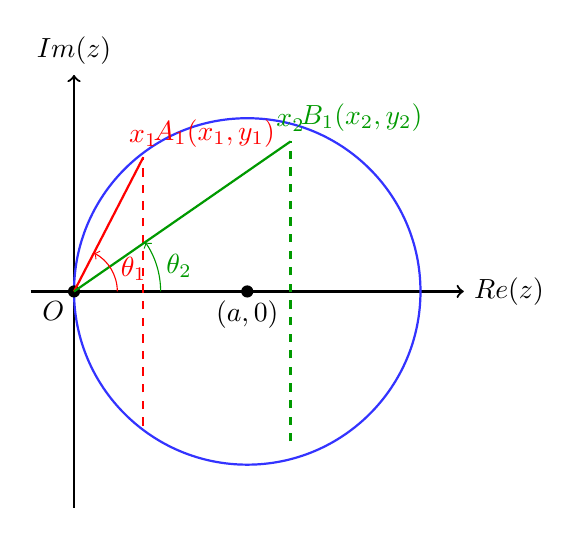
\begin{tikzpicture}[scale=1.1]
		\draw[->, thick] (-0.5,0) -- (4.5,0) node[right] {$\mathfrak{Re}(z)$};
		\draw[->, thick] (0,-2.5) -- (0,2.5) node[above] {$\mathfrak{Im}(z)$};
		\draw[thick, blue!80] (2,0) circle (2cm);
		\fill (2,0) circle (2pt) node[below] {$(a,0)$};
		\fill (0,0) circle (2pt) node[below left] {$O$};
		
		\draw[dashed, red, thick] (0.8,-1.549) -- (0.8,1.549) node[above] {$x_1$};
		\draw[dashed, green!60!black, thick] (2.5,-1.732) -- (2.5,1.732) node[above] {$x_2$};
		
		\draw[thick, red] (0,0) -- (0.8,1.549) node[above right] {$A_1(x_1,y_1)$};
		\draw[thick, green!60!black] (0,0) -- (2.5,1.732) node[above right] {$B_1(x_2,y_2)$};
		
		\draw[red, ->] (0.5,0) arc (0:62.68:0.5) node[midway, right] {$\theta_1$};
		\draw[green!60!black, ->] (1.0,0) arc (0:34.72:1.0) node[midway, right] {$\theta_2$};
	\end{tikzpicture}
	\caption{Geometric relationship between parallel chord $x$-intercepts ($x_1 < x_2$) and subtended ray angles ($\theta_1 > \theta_2$) for a circle tangent to the imaginary axis.}
	\label{fig:chord}
\end{figure}

\section{Decentralized Control Strategies for Loops excluding Leader/Root ($x_1 > 1$)}
When the root/leader node is external to the loop ($x_1 > 1$), Node 1 retains its zero in-degree property ($d_{\text{in},1} = 0$). We present three Gershgorin-based scaling strategies that guarantee consensus under fixed global coupling parameters $\gamma$.

\subsection{Node-Based Scaling Strategy}\label{sec:NodeMethod}
In Node-Based Scaling, the control law $u_i(t)$ of each agent participating in the cycle ($i \in \{x_1, x_1+1, \dots, y_1\}$) is scaled by a local positive scalar $p_{i-x_1+1} > 0$. Stacking these factors into a diagonal matrix $P = \text{diag}(p_1, p_2, \dots, p_{\ell+1}) \in \mathbb{R}^{(\ell+1) \times (\ell+1)}$, we construct the block diagonal network scaling matrix $\mathcal{D} \in \mathbb{R}^{N \times N}$:
\begin{equation} \label{eq:ch_GC_MatrixD}
	\mathcal{D} = \begin{bmatrix}
		I_{x_1-1} & 0 & 0 \\
		0 & P & 0 \\
		0 & 0 & I_{N-y_1}
	\end{bmatrix}
\end{equation}
\begin{figure}[ht!]
	\centering
	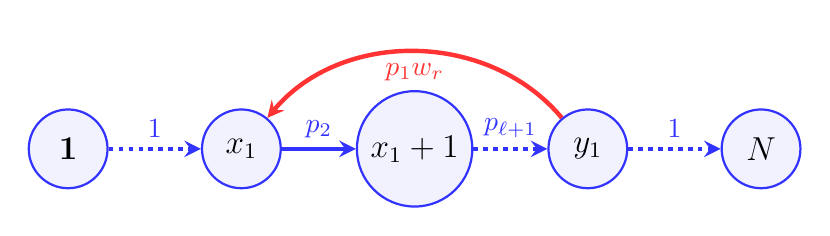
\begin{tikzpicture}[node distance=2.2cm, state/.style={circle, draw=blue!80, fill=blue!5, thick, minimum size=1.0cm, font=\large\bfseries}]
		\node[state] (1) {1};
		\node[state] (2) [right of=1] {$x_1$};
		\node[state] (3) [right of=2] {$x_1+1$};
		\node[state] (4) [right of=3] {$y_1$};
		\node[state] (5) [right of=4] {$N$};
		
		\path [->, >=stealth, ultra thick, blue!80] (1) edge[dotted] node[above] {$1$} (2);
		\path [->, >=stealth, ultra thick, blue!80] (2) edge node[above] {$p_2$} (3);
		\path [->, >=stealth, ultra thick, blue!80] (3) edge[dotted] node[above] {$p_{\ell+1}$} (4);
		\path [->, >=stealth, ultra thick, blue!80] (4) edge[dotted] node[above] {$1$} (5);
		\path [->, >=stealth, ultra thick, red!80] (4) edge[bend right=50] node[below] {$p_1 w_r$} (2);
	\end{tikzpicture}
	\caption{Node-Scaled Network Topology, where every incoming edge to node $i$ in the cycle is scaled by local scalar $p_{i-x_1+1}$.}
	\label{fig:NodeScaledNetwork}
\end{figure}

Premultiplying the modified Laplacian $\mathcal{L}_{\text{ext}}$ in \eqref{eq:ch_GC_OriginalLaplacian} by $\mathcal{D}$ yields the node-scaled equivalent Laplacian $\mathcal{L}_{\text{eq}} = \mathcal{D} \mathcal{L}_{\text{ext}}$:
\begin{equation} \label{eq:ch_GC_LaplacianEqNode}
	\mathcal{L}_{\text{eq}} = \begin{bmatrix}
		\mathcal{L}_1 & 0 & 0 \\
		* & P(\mathcal{C} + \mathcal{L}_{\text{re}}) & 0 \\
		* & * & \mathcal{L}_2
	\end{bmatrix}
\end{equation}
Defining $\tilde{P} \coloneqq P(\mathcal{C} + \mathcal{L}_{\text{re}}) \in \mathbb{R}^{(\ell+1) \times (\ell+1)}$, for an unweighted nominal chain with unit reverse edge ($w_r = 1$), $\tilde{P}$ takes the explicit tridiagonal-circulant form:
\begin{equation}\label{eq:ch_GC_NSChainLoop}
	\tilde{P} = \begin{bmatrix}
		2p_1  & 0 & 0 & \dots & 0 & -p_1 \\
		-p_2 & p_2 & 0 & \dots & 0 & 0 \\
		0 & -p_3 & p_3 & \dots & 0 & 0 \\
		\vdots & \vdots & \ddots & \ddots & \vdots & \vdots \\
		0 & 0 & \dots & -p_{\ell} & p_{\ell} & 0 \\
		0 & 0 & \dots & 0 & -p_{\ell+1} & p_{\ell+1}
	\end{bmatrix}
\end{equation}

Applying Gershgorin's Disc Theorem (Theorem \ref{thm:ch_GC_GershgorinDiscTheorem}) to the columns of $\tilde{P}$, column $j=1$ centered at $2p_1$ has radius $R_1 = p_2$. Columns $j \in \{2, \dots, \ell\}$ centered at $p_j$ have radii $R_j = p_{j+1}$. Column $j=\ell+1$ centered at $p_{\ell+1}$ has radius $R_{\ell+1} = p_1$. 

To guarantee that all column discs lie strictly in the open right half-plane $\mathfrak{Re}(z) > 0$, the center of each disc must strictly exceed its radius:
\begin{equation}\label{eq:ch_GC_NSInequality}
	2p_1 > p_2 > p_3 > \dots > p_{\ell+1} > p_1
\end{equation}

The left boundary of disc $j$ cuts the real axis at distance $d_j$ from the origin: $d_1 = 2p_1 - p_2$, $d_j = p_j - p_{j+1}$ for $j \in \{2, \dots, \ell\}$, and $d_{\ell+1} = p_{\ell+1} - p_1$. The minimum real separation across all discs is $J = \min_j (d_j)$. By Proposition \ref{prop:ch_GC_AP_optimization}, $J$ is maximized if and only if the centers $\{2p_1, p_2, \dots, p_{\ell+1}, p_1\}$ form an Arithmetic Progression (AP) with common difference:
\begin{equation}\label{eq:ch_GC_node_diff}
	d = \frac{2p_1 - p_1}{\ell + 1} = \frac{p_1}{\ell + 1}
\end{equation}

\begin{figure}[ht!]
	\centering
	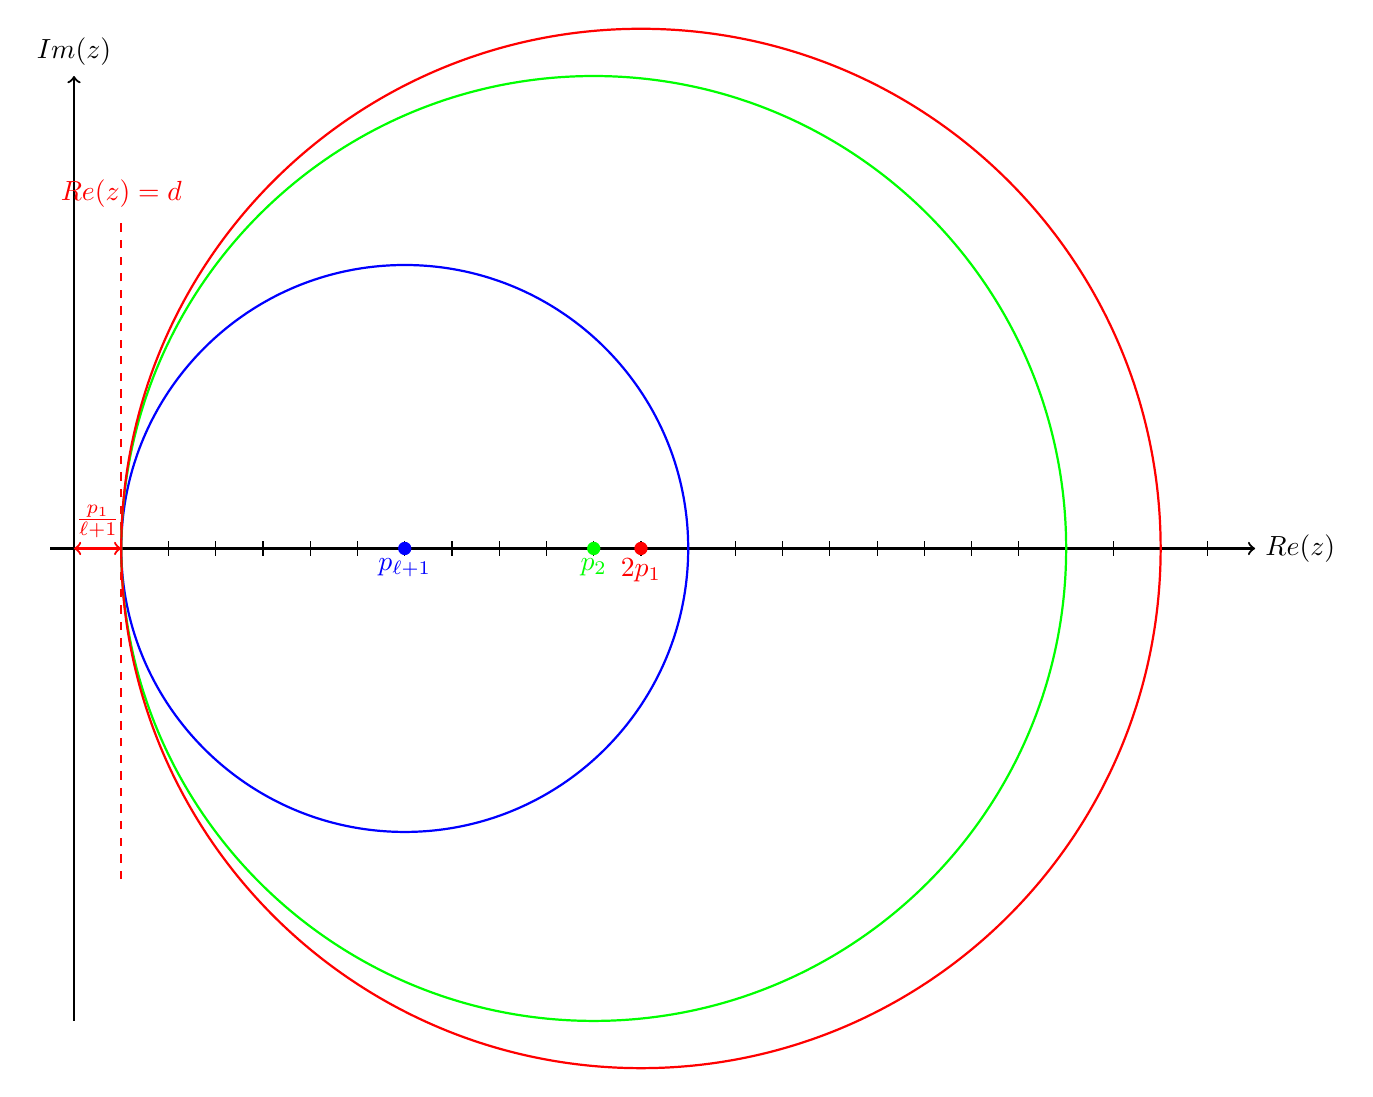
\begin{tikzpicture}[scale=0.3]
		\draw[->, thick] (-1,0) -- (50,0) node[right] {$\mathfrak{Re}(z)$};
		\draw[->, thick] (0,-20) -- (0,20) node[above] {$\mathfrak{Im}(z)$};
        \foreach \x in {2, 4, 6, 8, 10, 12, 14, 16, 18, 20, 22, 24, 26, 28, 30, 32, 34, 36, 38, 40, 42, 44, 46, 48}
		\draw[-] (\x, -0.3) -- (\x, 0.3);
		\draw[dashed, red, thick] (2,-14) -- (2,14) node[above] {$\mathfrak{Re}(z) = d$};
		
		\draw[draw=blue, thick] (14.0,0) circle (12cm);
		\fill[blue] (14.0,0) circle (8pt) node[below] {$p_{\ell+1}$};
		
		\draw[draw=green, thick] (22,0) circle (20.0cm);
		\fill[green] (22,0) circle (8pt) node[below] {$p_2$};
		
		\draw[draw=red, thick] (24.0,0) circle (22cm);
		\fill[red] (24.0,0) circle (8pt) node[below] {$2p_1$};
		
		\draw[<->, thick, red] (0,0) -- (2,0) node[midway, above] {$\frac{p_1}{\ell+1}$};
	\end{tikzpicture}
	\caption{Gershgorin column discs for $\tilde{P}$ when scaling parameters $p_i$ form an optimal Arithmetic Progression ($p_1 = 12, \ell = 5, d = 2$). All discs touch the boundary line $\mathfrak{Re}(z) = d$.}
	\label{fig:GersgorinDiscInAP}
\end{figure}
To ensure that the minimum spectral real part satisfies condition \eqref{eq:ch_GC_dubey_bound} ($\mathfrak{Re}(\lambda_2) \ge d \ge 1/\gamma^2$), we require $d = \frac{p_1}{\ell+1} \ge \frac{1}{\gamma^2} \implies p_1 \ge \frac{\ell+1}{\gamma^2}$. This establishes the following theorem:

\begin{theo}[Node-Based Scaling for Consensus Guarantee]\label{theo1}
Consider an $N$-node directed chain of double-integrator agents operating under protocol \eqref{eq:ch_GC_control_law} with fixed coupling $\gamma > 0$. Suppose a reverse edge of unit weight ($w_r = 1$) is inserted from node $y_1$ to node $x_1$ ($x_1 > 1$, range $\ell = y_1 - x_1$). Second-order consensus is guaranteed if the control law $u_i(t)$ of each node $i \in \{x_1, x_1+1, \dots, y_1\}$ is scaled by local factor $p_{i-x_1+1} > 0$:
\begin{equation}\label{eq:ch_GC_NodeScalar_formula}
	p_{i-x_1+1} = \left( \frac{\ell+1}{\gamma^2} + \epsilon \right) + (i - x_1) \frac{\frac{\ell+1}{\gamma^2} + \epsilon}{\ell + 1}, \quad \text{for any } \epsilon > 0
\end{equation}
\end{theo}

\begin{proof}
Substituting $p_1 = \frac{\ell+1}{\gamma^2} + \epsilon$ into \eqref{eq:ch_GC_node_diff} gives common difference $d = \frac{p_1}{\ell+1} = \frac{1}{\gamma^2} + \frac{\epsilon}{\ell+1} > \frac{1}{\gamma^2}$. By Proposition \ref{prop:ch_GC_AP_optimization}, constructing an AP with difference $d$ forces all column discs of $\tilde{P}$ to lie strictly to the right of $\mathfrak{Re}(z) = d$. By Gershgorin's Theorem, every non-zero eigenvalue satisfies $\mathfrak{Re}(\lambda_i) \ge d > 1/\gamma^2$. Substituting $\mathfrak{Re}(\lambda_2) > 1/\gamma^2$ into criterion \eqref{eq:ch_GC_dubey_bound} guarantees asymptotic state agreement.
\end{proof}


\subsection{Edge-Based Scaling Strategy}\label{sec:EdgeMethod}

Instead of scaling node dynamics, Edge-Based Scaling directly adjusts individual edge weights $w_k > 0$ for edges entering loop nodes. Let $w_1 > 0$ denote the forward edge weight entering head node $x_1$ from node $x_1 - 1$, let $w_r > 0$ be the reverse edge weight from $y_1$ to $x_1$, and let $\{w_2, w_3, \dots, w_{\ell+1}\}$ be the internal forward edge weights along the loop sub-chain (Figure \ref{fig:EdgeScaledNetwork}).

\begin{figure}[ht!]
	\centering
	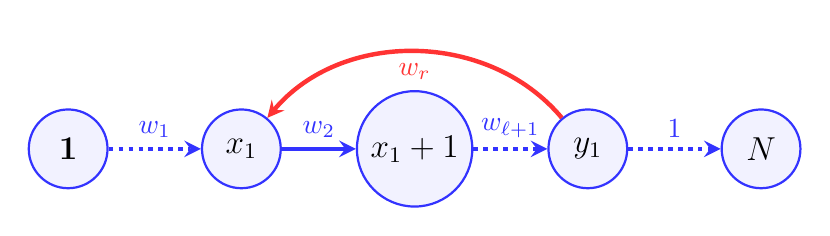
\begin{tikzpicture}[node distance=2.2cm, state/.style={circle, draw=blue!80, fill=blue!5, thick, minimum size=1.0cm, font=\large\bfseries}]
		\node[state] (1) {1};
		\node[state] (2) [right of=1] {$x_1$};
		\node[state] (3) [right of=2] {$x_1+1$};
		\node[state] (4) [right of=3] {$y_1$};
		\node[state] (5) [right of=4] {$N$};
		
		\path [->, >=stealth, ultra thick, blue!80] (1) edge[dotted] node[above] {$w_1$} (2);
		\path [->, >=stealth, ultra thick, blue!80] (2) edge node[above] {$w_2$} (3);
		\path [->, >=stealth, ultra thick, blue!80] (3) edge[dotted] node[above] {$w_{\ell+1}$} (4);
		\path [->, >=stealth, ultra thick, blue!80] (4) edge[dotted] node[above] {$1$} (5);
		\path [->, >=stealth, ultra thick, red!80] (4) edge[bend right=50] node[below] {$w_r$} (2);
	\end{tikzpicture}
	\caption{Edge-Scaled Network Topology, showing individual forward edge weight modifications $\{w_1, \dots, w_{\ell+1}\}$ along the feedback loop.}
	\label{fig:EdgeScaledNetwork}
\end{figure}

The sub-block matrix $\mathcal{C} + \mathcal{L}_{\text{re}}$ in \eqref{eq:ch_GC_OriginalLaplacian} takes the weighted form:
\begin{equation}\label{eq:ch_GC_ESChainLoop}
	\mathcal{C} + \mathcal{L}_{\text{re}} = \begin{bmatrix}
		w_1 + w_r  & 0 & \dots & 0 & -w_r \\
		-w_2 & w_2 & \dots & 0 & 0 \\
		0 & -w_3 & \dots & 0 & 0 \\
		\vdots & \vdots & \ddots & \vdots & \vdots \\
		0 & 0 & \dots & -w_{\ell+1} & w_{\ell+1}
	\end{bmatrix}
\end{equation}

Applying Gershgorin's Theorem to the columns of \eqref{eq:ch_GC_ESChainLoop}, disc 1 is centered at $w_1 + w_r$ with radius $w_2$, discs $k \in \{2, \dots, \ell\}$ are centered at $w_k$ with radii $w_{k+1}$, and disc $\ell+1$ is centered at $w_{\ell+1}$ with radius $w_r$. Ensuring all discs lie in $\mathfrak{Re}(z) > 0$ requires:
\begin{equation}\label{eq:ch_GC_ESInequality}
	w_1 + w_r > w_2 > w_3 > \dots > w_{\ell+1} > w_r
\end{equation}

By Proposition \ref{prop:ch_GC_AP_optimization}, creating an AP between $w_1 + w_r$ and $w_r$ maximizes the minimum separation $d = \frac{(w_1 + w_r) - w_r}{\ell + 1} = \frac{w_1}{\ell + 1}$. Setting $d = \frac{w_1}{\ell + 1} \ge \frac{1}{\gamma^2} \implies w_1 \ge \frac{\ell+1}{\gamma^2}$ which yields the following edge-scaling theorem:

\begin{theo}[Edge-Based Scaling for Consensus Guarantee]\label{theo2}
Consider an $N$-node directed chain of double integrators operating under protocol \eqref{eq:ch_GC_control_law} with fixed coupling $\gamma > 0$. Suppose a reverse edge of weight $w_r > 0$ is added from $y_1$ to $x_1$ ($x_1 > 1$, range $\ell$). Second-order consensus is guaranteed if forward edge weights $\{w_1, w_2, \dots, w_{\ell+1}\}$ are tuned as:
\begin{equation}\label{eq:ch_GC_ESScalar_formula}
	w_1 = \frac{\ell+1}{\gamma^2} + \epsilon, \quad w_k = w_1 + (k-1) \frac{w_1}{\ell+1}, \quad \text{for any } \epsilon > 0, k \in \{2, \dots, \ell+1\}
\end{equation}
\end{theo}

\begin{remark}[Asymmetric Sensitivity of Edge Weight Tuning]\label{rem:ch_GC_EdgeChoice}
Equation \eqref{eq:ch_GC_ESScalar_formula} demonstrates that the common difference $d = w_1 / (\ell+1)$ depends strictly on $w_1$ (the forward edge weight entering head node $x_1$ from exterior node $x_1 - 1$) and is completely independent of the reverse edge weight $w_r$. Increasing $w_1$ strengthens the authority of the upstream leader sub-chain over the loop, whereas increasing $w_r$ strengthens internal cycle feedback, degrading stability.
\end{remark}

\subsection{Combined Node-Edge Scaling Strategy}\label{sec:combo}

Combined Scaling merges node scaling factors $P = \text{diag}(p_1, \dots, p_{\ell+1})$ with edge weights $\{w_1, \dots, w_{\ell+1}\}$ to form $\tilde{P} = P(\mathcal{C} + \mathcal{L}_{\text{re}})$:
\begin{equation}\label{eq:ch_GC_eqcombined}
	\tilde{P} = \begin{bmatrix}
		p_1(w_1 + w_r)  & 0 & \dots & -p_1 w_r \\
		-p_2 w_2 & p_2 w_2 & \dots & 0 \\
		\vdots & \vdots & \ddots & \vdots \\
		0 & 0 & \dots & p_{\ell+1} w_{\ell+1}
	\end{bmatrix}
\end{equation}

Constructing an AP between $p_1(w_1 + w_r)$ and $p_1 w_r$ leads to a common difference of $d = \frac{p_1(w_1 + w_r) - p_1 w_r}{\ell + 1} = \frac{p_1 w_1}{\ell + 1}$. Setting $d \ge \frac{1}{\gamma^2} \implies p_1 w_1 \ge \frac{\ell+1}{\gamma^2}$ which yields the following result:

\begin{theo}[Combined Scaling for Consensus Guarantee]\label{theo3}
\leavevmode\par\noindent
Second-order consensus is guaranteed under protocol \eqref{eq:ch_GC_control_law} with fixed coupling $\gamma > 0$ if node factors $p_i$ and edge weights $w_i$ are selected such that:
\begin{equation}
	p_1 w_1 = \frac{\ell+1}{\gamma^2} + \epsilon, \quad p_i w_i = p_1 w_1 + (i-1) \frac{p_1 w_1}{\ell+1}, \quad \text{for } \epsilon > 0, i \in \{2, \dots, \ell+1\}
\end{equation}
\end{theo}

\begin{remark}[Implementation Flexibility of Combined Scaling]\label{rem:ch_GC_combined_flexibility}
Combined Scaling allows hardware trade-offs between node gain amplification ($p_1$) and physical edge weight adjustments ($w_1$). In physical deployments, setting $p_i = p_1$ uniformly across all cycle nodes allows edge weights $w_i$ to be adjusted within the practical bounded hardware range $w_i \in [1, 2]$.
\end{remark}


\section{Root-Locus Design Method for Loops involving the Root-Node ($x_1 = 1$)}\label{sec:ch_GC_RootLocusMethod}

When the reverse edge terminates at Node 1 itself ($x_1 = 1$, Figure \ref{fig:LeaderCycleNetwork}), Node 1 loses its zero in-degree property ($d_{\text{in}, 1} = w_r > 0$). Matrix $\mathcal{C} + \mathcal{L}_{\text{re}}$ in \eqref{eq:ch_GC_OriginalLaplacianleader} becomes a circulant-like matrix containing the zero eigenvalue $\lambda_1 = 0$. 

Under Gershgorin analysis, the column centers satisfy $2p_1, p_2, \dots, p_{\ell+1}$, but column $\ell+1$ has radius $p_1$, forcing condition $p_1 > p_2 > \dots > p_{\ell+1} > p_1$, which is impossible to satisfy. Thus, Gershgorin-based disc separation fails entirely for root-node loops.

To resolve this structural singularity, we formulate a complementary root-locus control framework.

\subsection{Complementary Root-Locus Formulation}

Suppose the control dynamics of all nodes in the root loop $\{1, 2, \dots, y_1\}$ are scaled by node factor $\alpha > 0$. Additionally, let the forward edge weight connecting Node 1 to Node 2 be scaled by edge factor $\beta / \alpha > 0$, where $\alpha$ and $\beta$ are design parameters. The loop sub-block matrix $\mathcal{C} + \mathcal{L}_{\text{re}} \in \mathbb{R}^{(\ell+1) \times (\ell+1)}$ takes the form:
\begin{equation}\label{eq:ch_GC_scaledmatrix}
	\mathcal{C} + \mathcal{L}_{\text{re}} = \begin{bmatrix}
		\alpha  & 0 & 0 & \dots & -\alpha \\
		-\beta & \beta & 0 & \dots & 0 \\
		0 & -\alpha & \alpha & \dots & 0 \\
		\vdots & \vdots & \ddots & \ddots & \vdots \\
		0 & 0 & \dots & -\alpha & \alpha
	\end{bmatrix}
\end{equation}

Computing the characteristic polynomial of \eqref{eq:ch_GC_scaledmatrix}:
\begin{equation}\label{eq:ch_GC_chareq}
	(s - \alpha)^\ell (s - \beta) + (-1)^\ell \alpha^\ell \beta = 0
\end{equation}
Rearranging \eqref{eq:ch_GC_chareq} into standard $1 + K G(s) = 0$ feedback form:
\begin{equation}\label{eq:ch_GC_rearrangedchar}
	1 + \beta \cdot G(s) = 0, \quad \text{where } G(s) \coloneqq \frac{(s - \alpha)^\ell - (-\alpha)^\ell}{s (s - \alpha)^\ell}
\end{equation}

\begin{figure}[ht!]
	\centering
	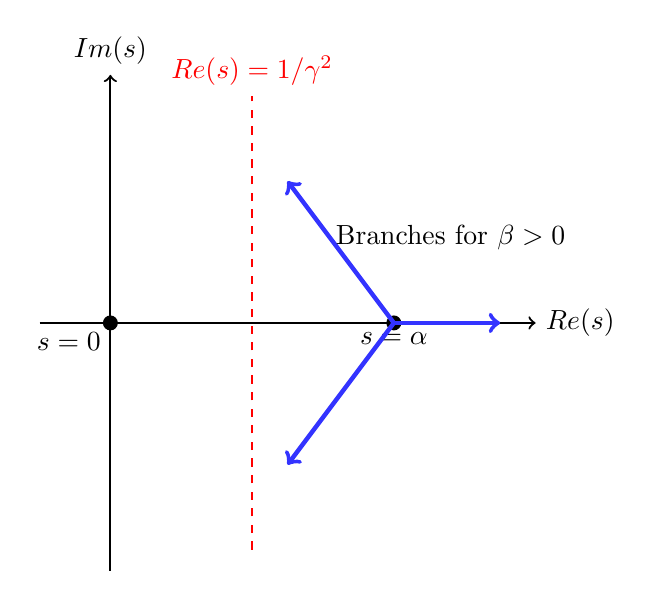
\begin{tikzpicture}[scale=0.9]
		\draw[->, thick] (-1,0) -- (6,0) node[right] {$\mathfrak{Re}(s)$};
		\draw[->, thick] (0,-3.5) -- (0,3.5) node[above] {$\mathfrak{Im}(s)$};
		
		\fill (0,0) circle (3pt) node[below left] {$s=0$};
		\fill (4,0) circle (3pt) node[below] {$s=\alpha$};
		
		\draw[dashed, red, thick] (2, -3.2) -- (2, 3.2) node[above] {$\mathfrak{Re}(s) = 1/\gamma^2$};
		
		\draw[ultra thick, blue!80, ->] (4,0) -- (2.5, 2.0);
		\draw[ultra thick, blue!80, ->] (4,0) -- (2.5, -2.0);
		\draw[ultra thick, blue!80, ->] (4,0) -- (5.5, 0);
		
		\node at (4.8, 1.2) {Branches for $\beta > 0$};
	\end{tikzpicture}
	\caption{Complementary Root-Locus trajectory of $G(s)$ for fixed $\alpha > 1/\gamma^2$ as gain $\beta$ increases from 0. Branches emanate from pole $s = \alpha$ toward the imaginary axis.}
	\label{fig:RootLocusBasedNetwork}
\end{figure}

The open-loop poles of $G(s)$ reside at $s = 0$ (simple) and $s = \alpha$ (multiplicity $\ell$). The open-loop zeros reside at $s = \alpha \left( 1 + e^{j \frac{\pi}{\ell}(2k+1)} \right)$ for odd $\ell$, and $s = \alpha \left( 1 + e^{j \frac{\pi}{\ell}(2k)} \right)$ for even $\ell$. Note that $G(s)$ possesses a pole-zero cancellation at the origin $s = 0$.

For $\beta = 0$, all non-zero roots reside at $s = \alpha$. As gain $\beta > 0$ increases, root locus branches emanate from $s = \alpha$ and head toward the imaginary axis (Figure \ref{fig:RootLocusBasedNetwork}). To preserve consensus under fixed coupling $\gamma$, we select $\alpha > 1/\gamma^2$ and bound gain $\beta$ such that no root branch crosses to the left of $\mathfrak{Re}(z) = 1/\gamma^2$:

\begin{theo}[Root-Locus based Gain Scaling for Consensus Guarantee]\label{theo3ES}
\leavevmode\par\noindent
Consider an $N$-node directed chain of double integrators operating under protocol \eqref{eq:ch_GC_control_law} with fixed coupling $\gamma > 0$. Suppose a reverse edge is added from $y_1$ to $x_1 = 1$ ($x_1 = 1$, range $\ell$). Select node scaling factor $\alpha > 1/\gamma^2$. Then, there exists a upper gain bound $\bar{\beta} > 0$ such that when the control law of one agent in the loop is scaled by $\beta / \alpha$ (with $0 < \beta < \bar{\beta}$), second-order consensus is guaranteed.
\end{theo}

\begin{proof}
For $\beta = 0$, the non-zero roots of \eqref{eq:ch_GC_chareq} reside at $s = \alpha > 1/\gamma^2$, satisfying condition \eqref{eq:ch_GC_dubey_bound}. By root continuity with respect to parameter variations, for any $\alpha > 1/\gamma^2$, there exists $\bar{\beta} > 0$ such that for all $0 < \beta < \bar{\beta}$, all non-zero roots satisfy $\mathfrak{Re}(s_i) \ge 1/\gamma^2$, guaranteeing consensus.
\end{proof}

\subsection{Single-Gain Cyclic Pursuit Synthesis (One Cycle, One Gain)}

To prevent edge-weakening ($\beta \to 0$) when root-node forms a part of the loop, we synthesize an equal-weight cyclic pursuit design where all edges in the cycle share an identical weight $\alpha > 0$.

\begin{theo}[Single-Gain Threshold for Root-Node Loops]\label{theoonegain}
\leavevmode\par\noindent
Consider an $N$-agent double-integrator network containing a root-node loop of range $\ell$ with equal edge weights $\alpha > 0$. Second-order consensus is guaranteed under fixed coupling parameter $\gamma > 0$ if $\alpha$ satisfies:
\begin{equation}\label{eq:ch_GC_onegain_bound}
	\alpha \ge \frac{\cot^2\left(\frac{\pi}{\ell+1}\right)}{2\gamma^2}
\end{equation}
\end{theo}

\begin{proof}
For an $(\ell+1)$-node cyclic pursuit graph with equal edge weights $\alpha$, the characteristic equation is $(s + \alpha)^{\ell+1} = \alpha^{\ell+1}$. The roots are:
\begin{equation}\label{eq:ch_GC_rootsunity}
	s_k = \alpha \left( e^{j \frac{2\pi k}{\ell+1}} - 1 \right), \quad k \in \{0, 1, \dots, \ell\}
\end{equation}
The non-zero eigenvalues of the Laplacian $\mathcal{L}_{\text{root}}$ are $\lambda_k = -s_k = \alpha \left( 1 - e^{j \frac{2\pi k}{\ell+1}} \right)$. All non-zero eigenvalues lie on a circle of radius $\alpha$ centered at $(\alpha, 0)$ in the complex plane, tangent to the imaginary axis at the origin (Figure \ref{fig:SineAngle}).

\begin{figure}[ht!]
	\centering
	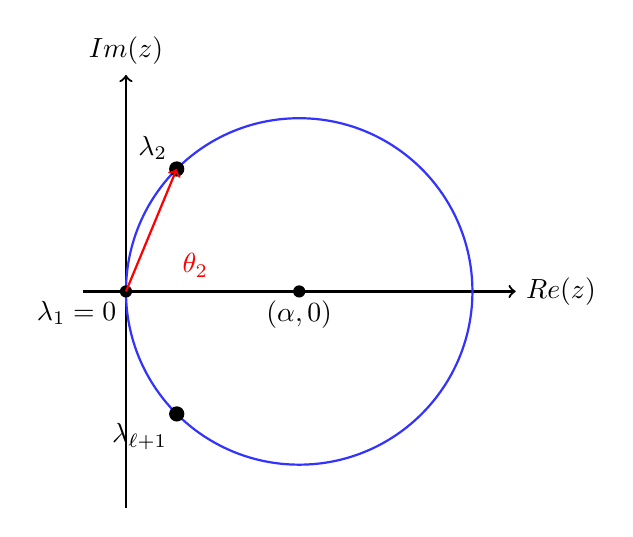
\begin{tikzpicture}[scale=1.1]
		\draw[->, thick] (-0.5,0) -- (4.5,0) node[right] {$\mathfrak{Re}(z)$};
		\draw[->, thick] (0,-2.5) -- (0,2.5) node[above] {$\mathfrak{Im}(z)$};
		\draw[thick, blue!80] (2,0) circle (2cm);
		\fill (2,0) circle (2pt) node[below] {$(\alpha,0)$};
		\fill (0,0) circle (2pt) node[below left] {$\lambda_1=0$};
		
		\fill (0.586, 1.414) circle (2.5pt) node[above left] {$\lambda_2$};
		\fill (0.586, -1.414) circle (2.5pt) node[below left] {$\lambda_{\ell+1}$};
		\draw[thick, red, ->] (0,0) -- (0.586, 1.414);
		\draw[red] (0.8, 0.3) node {$\theta_2$};
	\end{tikzpicture}
	\caption{Eigenvalue distribution of an $(\ell+1)$-node equal-weight cyclic pursuit Laplacian on a circle of radius $\alpha$. Eigenvalue $\lambda_2$ (corresponding to $k=1$) subtends the maximum ray angle $\theta_2$.}
	\label{fig:SineAngle}
\end{figure}

The necessary and sufficient consensus condition \eqref{eq:ch_GC_yu_threshold_recap} can be re-written in polar form as $\gamma \ge \max_k \frac{\sin \theta_k}{\sqrt{\mathfrak{Re}(\lambda_k)}}$, where $\theta_k$ is the ray angle subtended by $\lambda_k$ at the origin. By Proposition \ref{prop:ch_GC_chord_geometry}, the eigenvalue closest to the origin ($\lambda_2$, corresponding to $k=1$) subtends the maximum ray angle $\theta_2 = \frac{\pi}{2} - \frac{\pi}{\ell+1}$. 

Computing $\mathfrak{Re}(\lambda_2) = \alpha \left( 1 - \cos\left(\frac{2\pi}{\ell+1}\right) \right) = 2\alpha \sin^2\left(\frac{\pi}{\ell+1}\right)$ and $\sin(\theta_2) = \cos\left(\frac{\pi}{\ell+1}\right)$:
\begin{equation}
	\frac{\sin \theta_2}{\sqrt{\mathfrak{Re}(\lambda_2)}} = \frac{\cos\left(\frac{\pi}{\ell+1}\right)}{\sqrt{2\alpha \sin^2\left(\frac{\pi}{\ell+1}\right)}} = \frac{\cot\left(\frac{\pi}{\ell+1}\right)}{\sqrt{2\alpha}}
\end{equation}
Substituting this expression into $\gamma \ge \frac{\sin \theta_2}{\sqrt{\mathfrak{Re}(\lambda_2)}}$:
\begin{equation}
	\gamma \ge \frac{\cot\left(\frac{\pi}{\ell+1}\right)}{\sqrt{2\alpha}} \implies \gamma^2 \ge \frac{\cot^2\left(\frac{\pi}{\ell+1}\right)}{2\alpha} \implies \alpha \ge \frac{\cot^2\left(\frac{\pi}{\ell+1}\right)}{2\gamma^2}
\end{equation}
which completes the proof.
\end{proof}

\section{Numerical Simulations}\label{sec:ch_GC_simulations}
To demonstrate the efficacy of the proposed localized remedies, simulations were conducted on a 10-agent network ($N = 10$) governed by double-integrator dynamics with a predesigned velocity coupling parameter $\gamma = 0.5$.
A reverse edge of unit weight ($w_r = 1$) is inserted from node $y_1 = 9$ to node $x_1 = 3$, creating a feedback loop of range $\ell = y_1 - x_1 = 6$. The unperturbed nominal chain operates under Laplacian $\mathcal{L}$. With the reverse edge added, the modified sub-block $\mathcal{C} + \mathcal{L}_{\text{re}}$ (spanning nodes 3 through 9) takes the 7-dimensional form:
\begin{equation} \label{eq:ch_GC_ExampleLaplacian_block}
	\mathcal{C} + \mathcal{L}_{\text{re}} = \begin{bmatrix}
		2 & 0 & 0 & 0 & 0 & 0 & -1 \\
		-1 & 1 & 0 & 0 & 0 & 0 & 0 \\
		0 & -1 & 1 & 0 & 0 & 0 & 0 \\
		0 & 0 & -1 & 1 & 0 & 0 & 0 \\
		0 & 0 & 0 & -1 & 1 & 0 & 0 \\
		0 & 0 & 0 & 0 & -1 & 1 & 0 \\
		0 & 0 & 0 & 0 & 0 & -1 & 1
	\end{bmatrix}
\end{equation}
Under the unperturbed reverse edge, applying Yu's exact threshold \eqref{eq:ch_GC_yu_threshold_recap} reveals that the modified network requires $\gamma \ge 1.2134$. Because the predesigned global parameter is fixed at $\gamma = 0.5 < 1.2134$, consensus breaks down completely, as demonstrated by the diverging position and velocity trajectories in Figures \ref{fig:10-9-3_OriginalLaplacianGamma0.5PositionConsensus} and \ref{fig:10-9-3_OriginalLaplacianGamma0.5VelocityConsensus}. If $\gamma$ were retuned globally to $\gamma = 1.5$, consensus would be restored (Figures \ref{fig:10-9-3_OriginalLaplacianGamma1.5PositionConsensus} and \ref{fig:10-9-3_OriginalLaplacianGamma1.5VelocityConsensus}), but this requires global access to the Laplacian spectrum of the graph that results from the addition of the reverse edge.
\begin{figure}[ht!]
	\centering
	\begin{subfigure}[b]{1.0\textwidth}
		\centering
		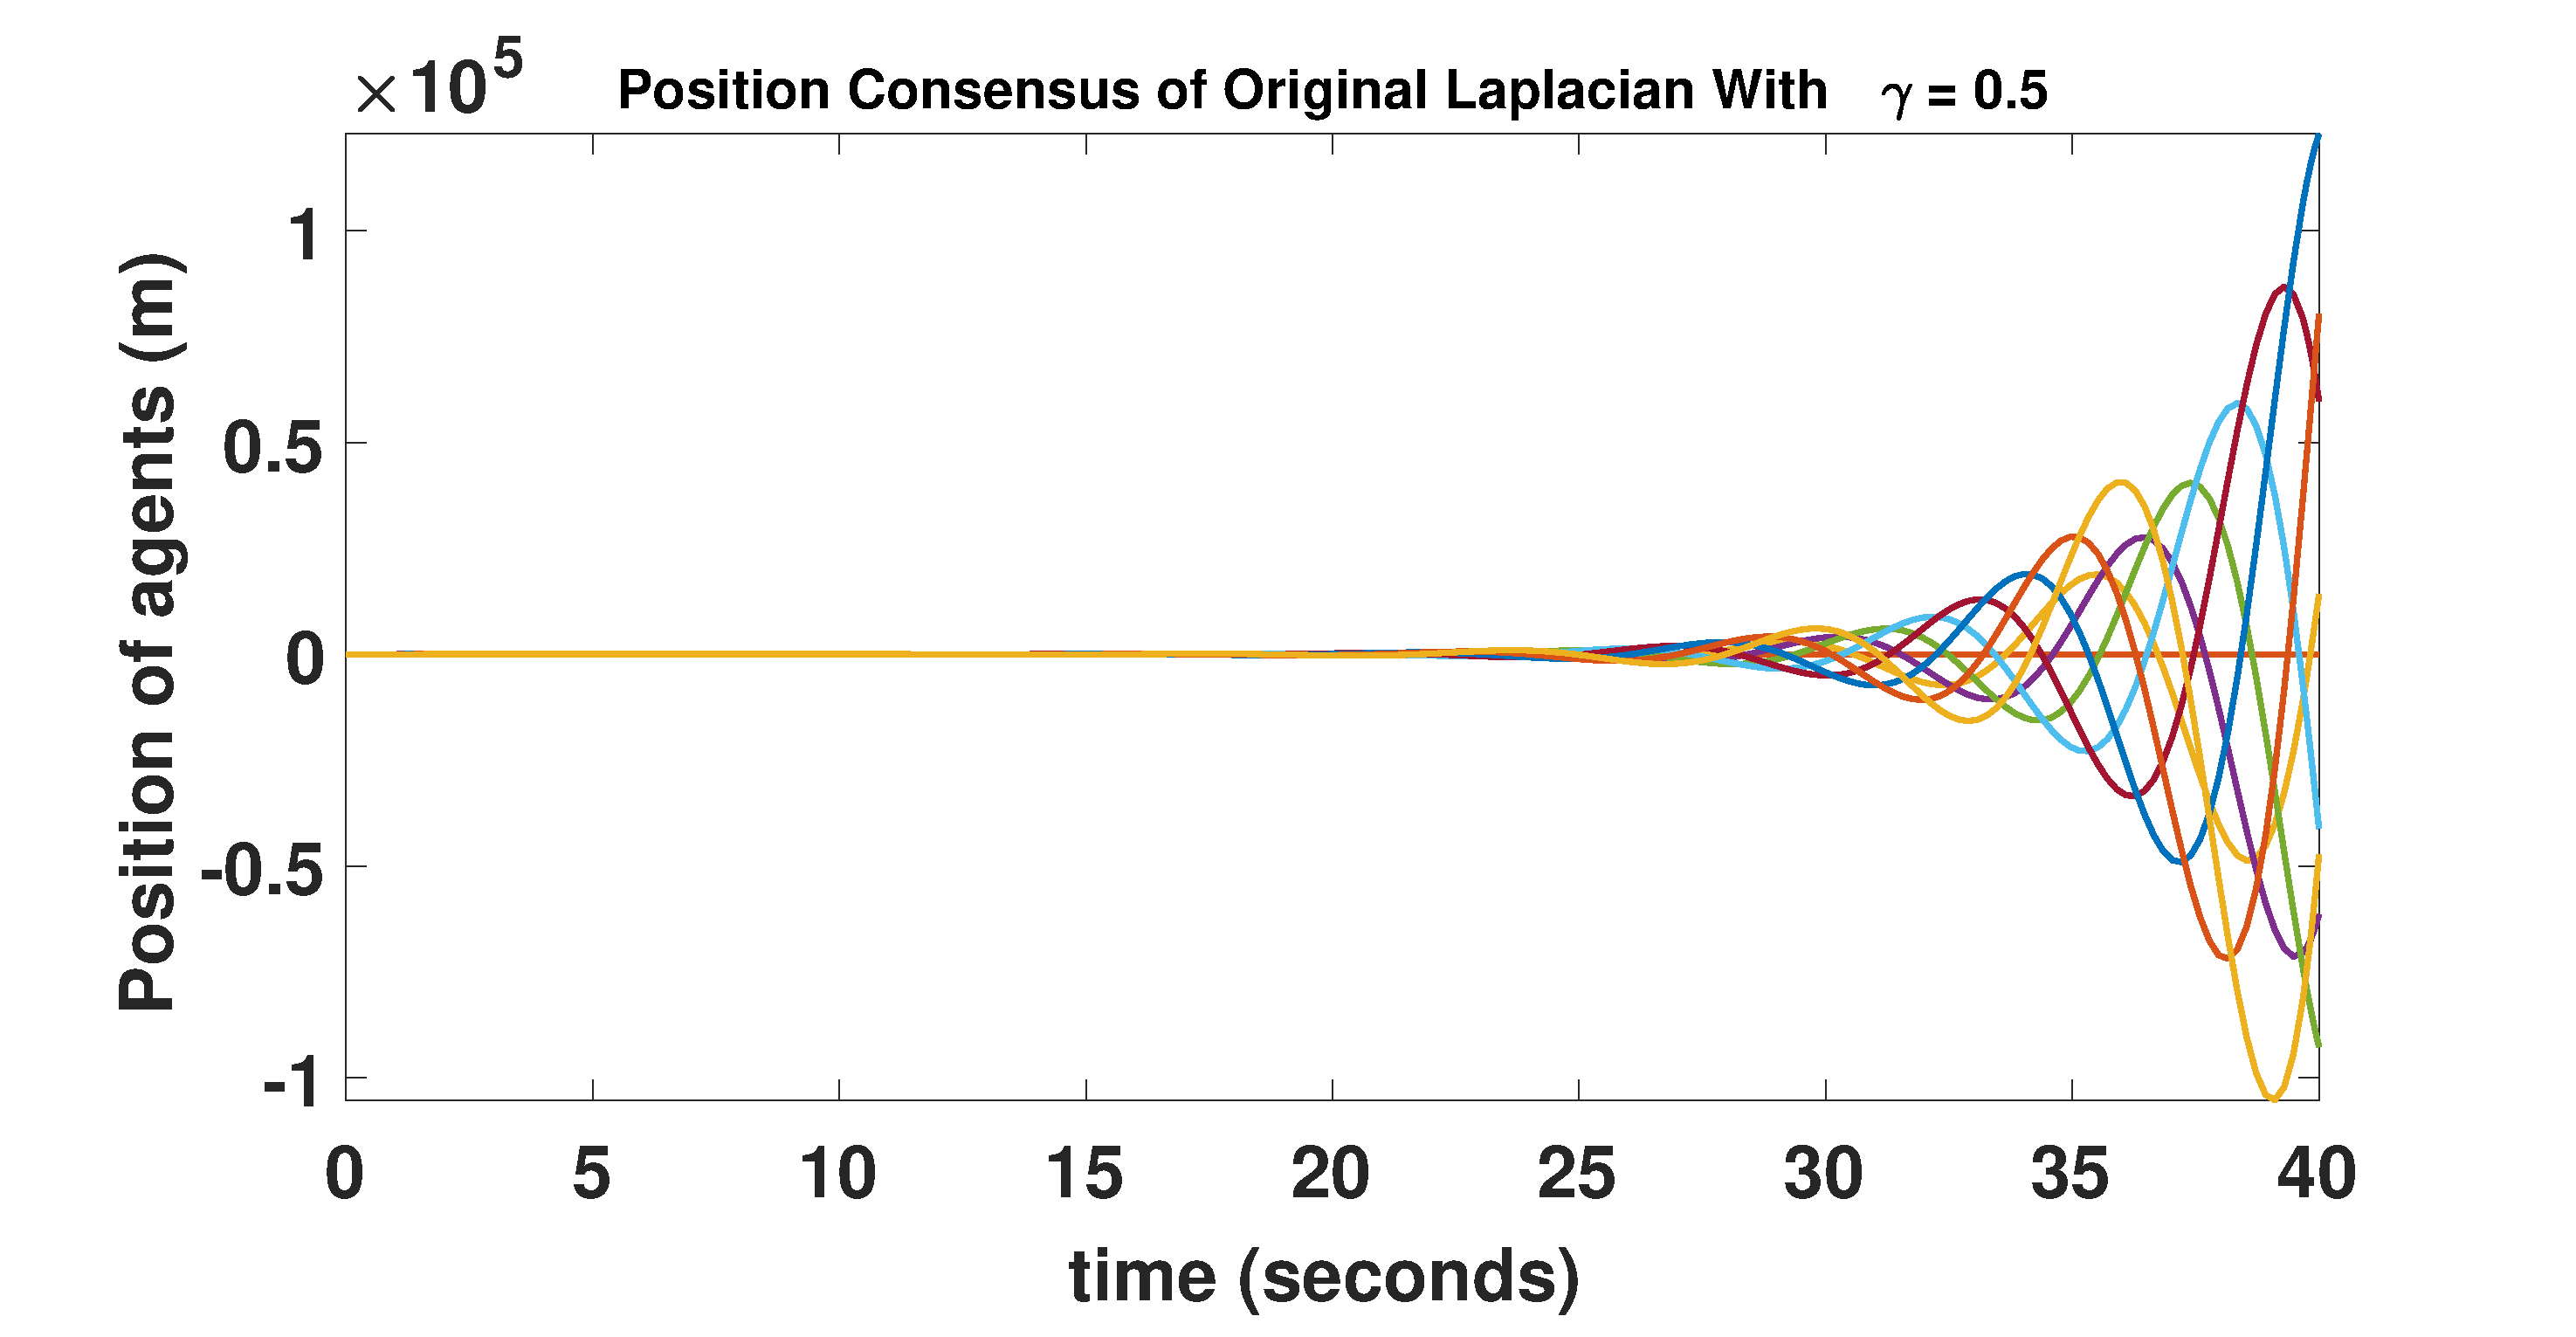
\includegraphics[width=\textwidth, keepaspectratio]{3_Images/10-9-3_OriginalLaplacianGamma0.5PositionConsensus.eps}
		\caption{Position trajectory divergence ($\gamma = 0.5$).}
		\label{fig:10-9-3_OriginalLaplacianGamma0.5PositionConsensus}
	\end{subfigure}
	
	\vspace{1em} % Adds vertical separation between stacked subfigures
	
	\begin{subfigure}[b]{1.0\textwidth}
		\centering
		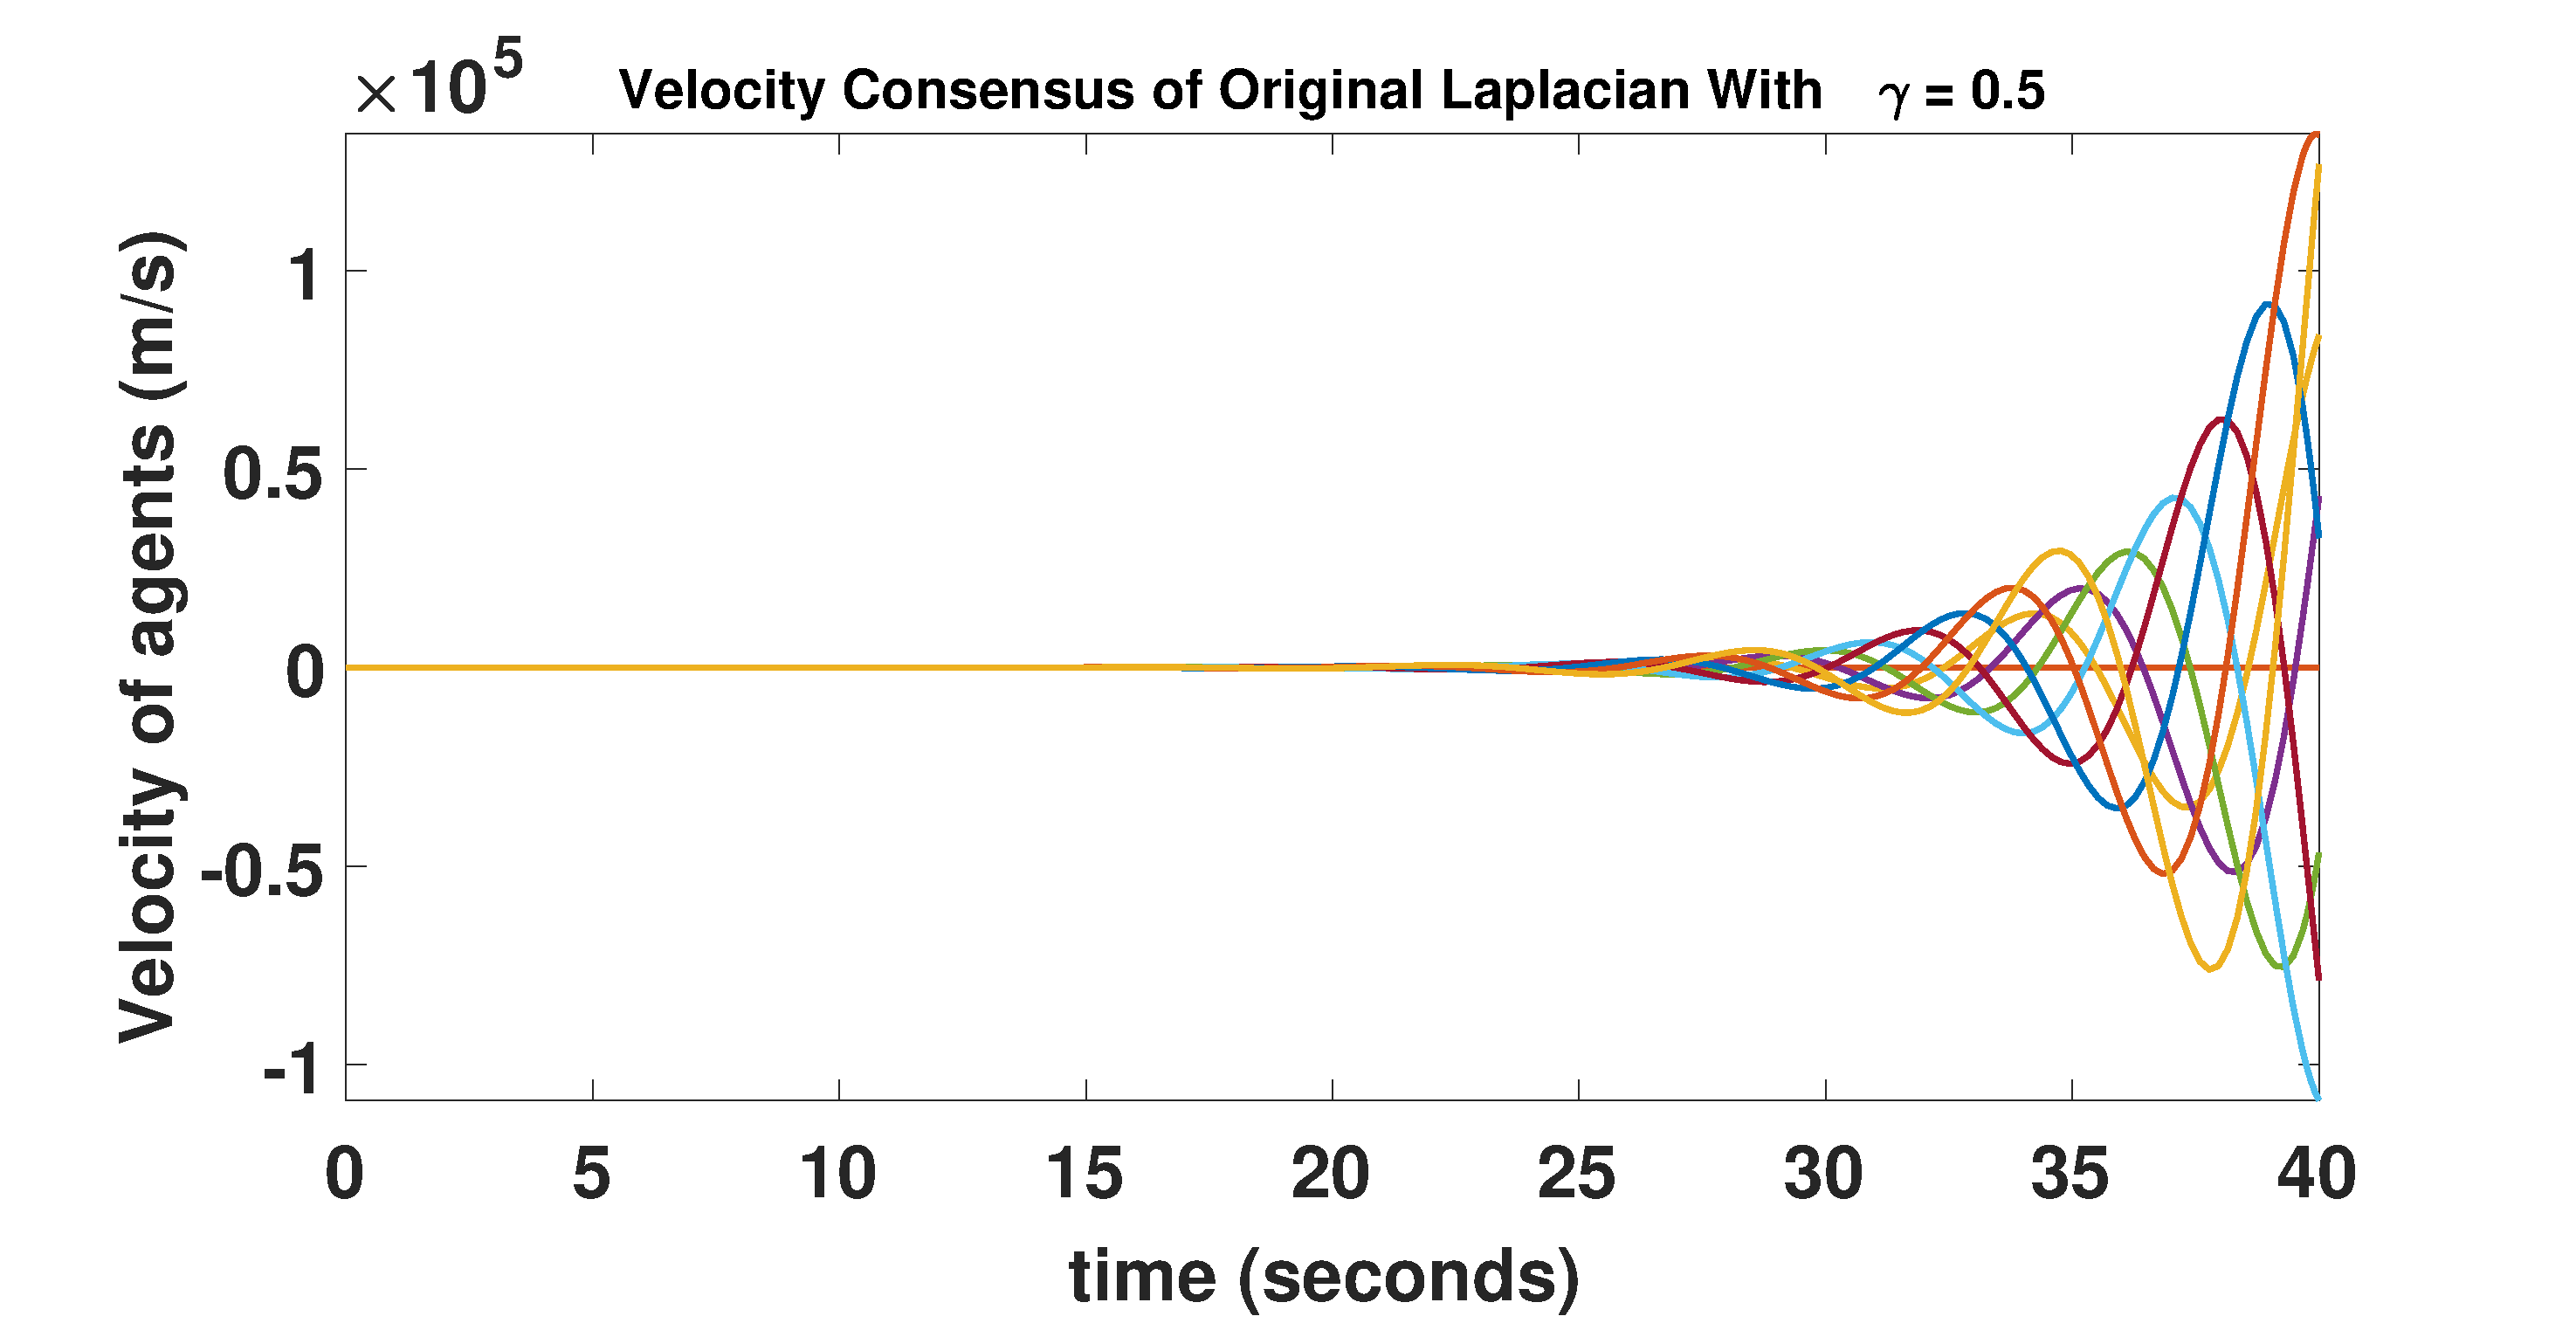
\includegraphics[width=\textwidth, keepaspectratio]{3_Images/10-9-3_OriginalLaplacianGamma0.5VelocityConsensus.eps}
		\caption{Velocity trajectory divergence ($\gamma = 0.5$).}
		\label{fig:10-9-3_OriginalLaplacianGamma0.5VelocityConsensus}
	\end{subfigure}
	\caption{Consensus breakdown in a 10-agent network under unperturbed reverse edge ($y_1=9, x_1=3, \ell=6$) when fixed coupling $\gamma = 0.5 < 1.2134$.}
	\label{fig:unperturbed_breakdown}
\end{figure}

\begin{figure}[ht!]
	\centering
	\begin{subfigure}[b]{\textwidth}
		\centering
		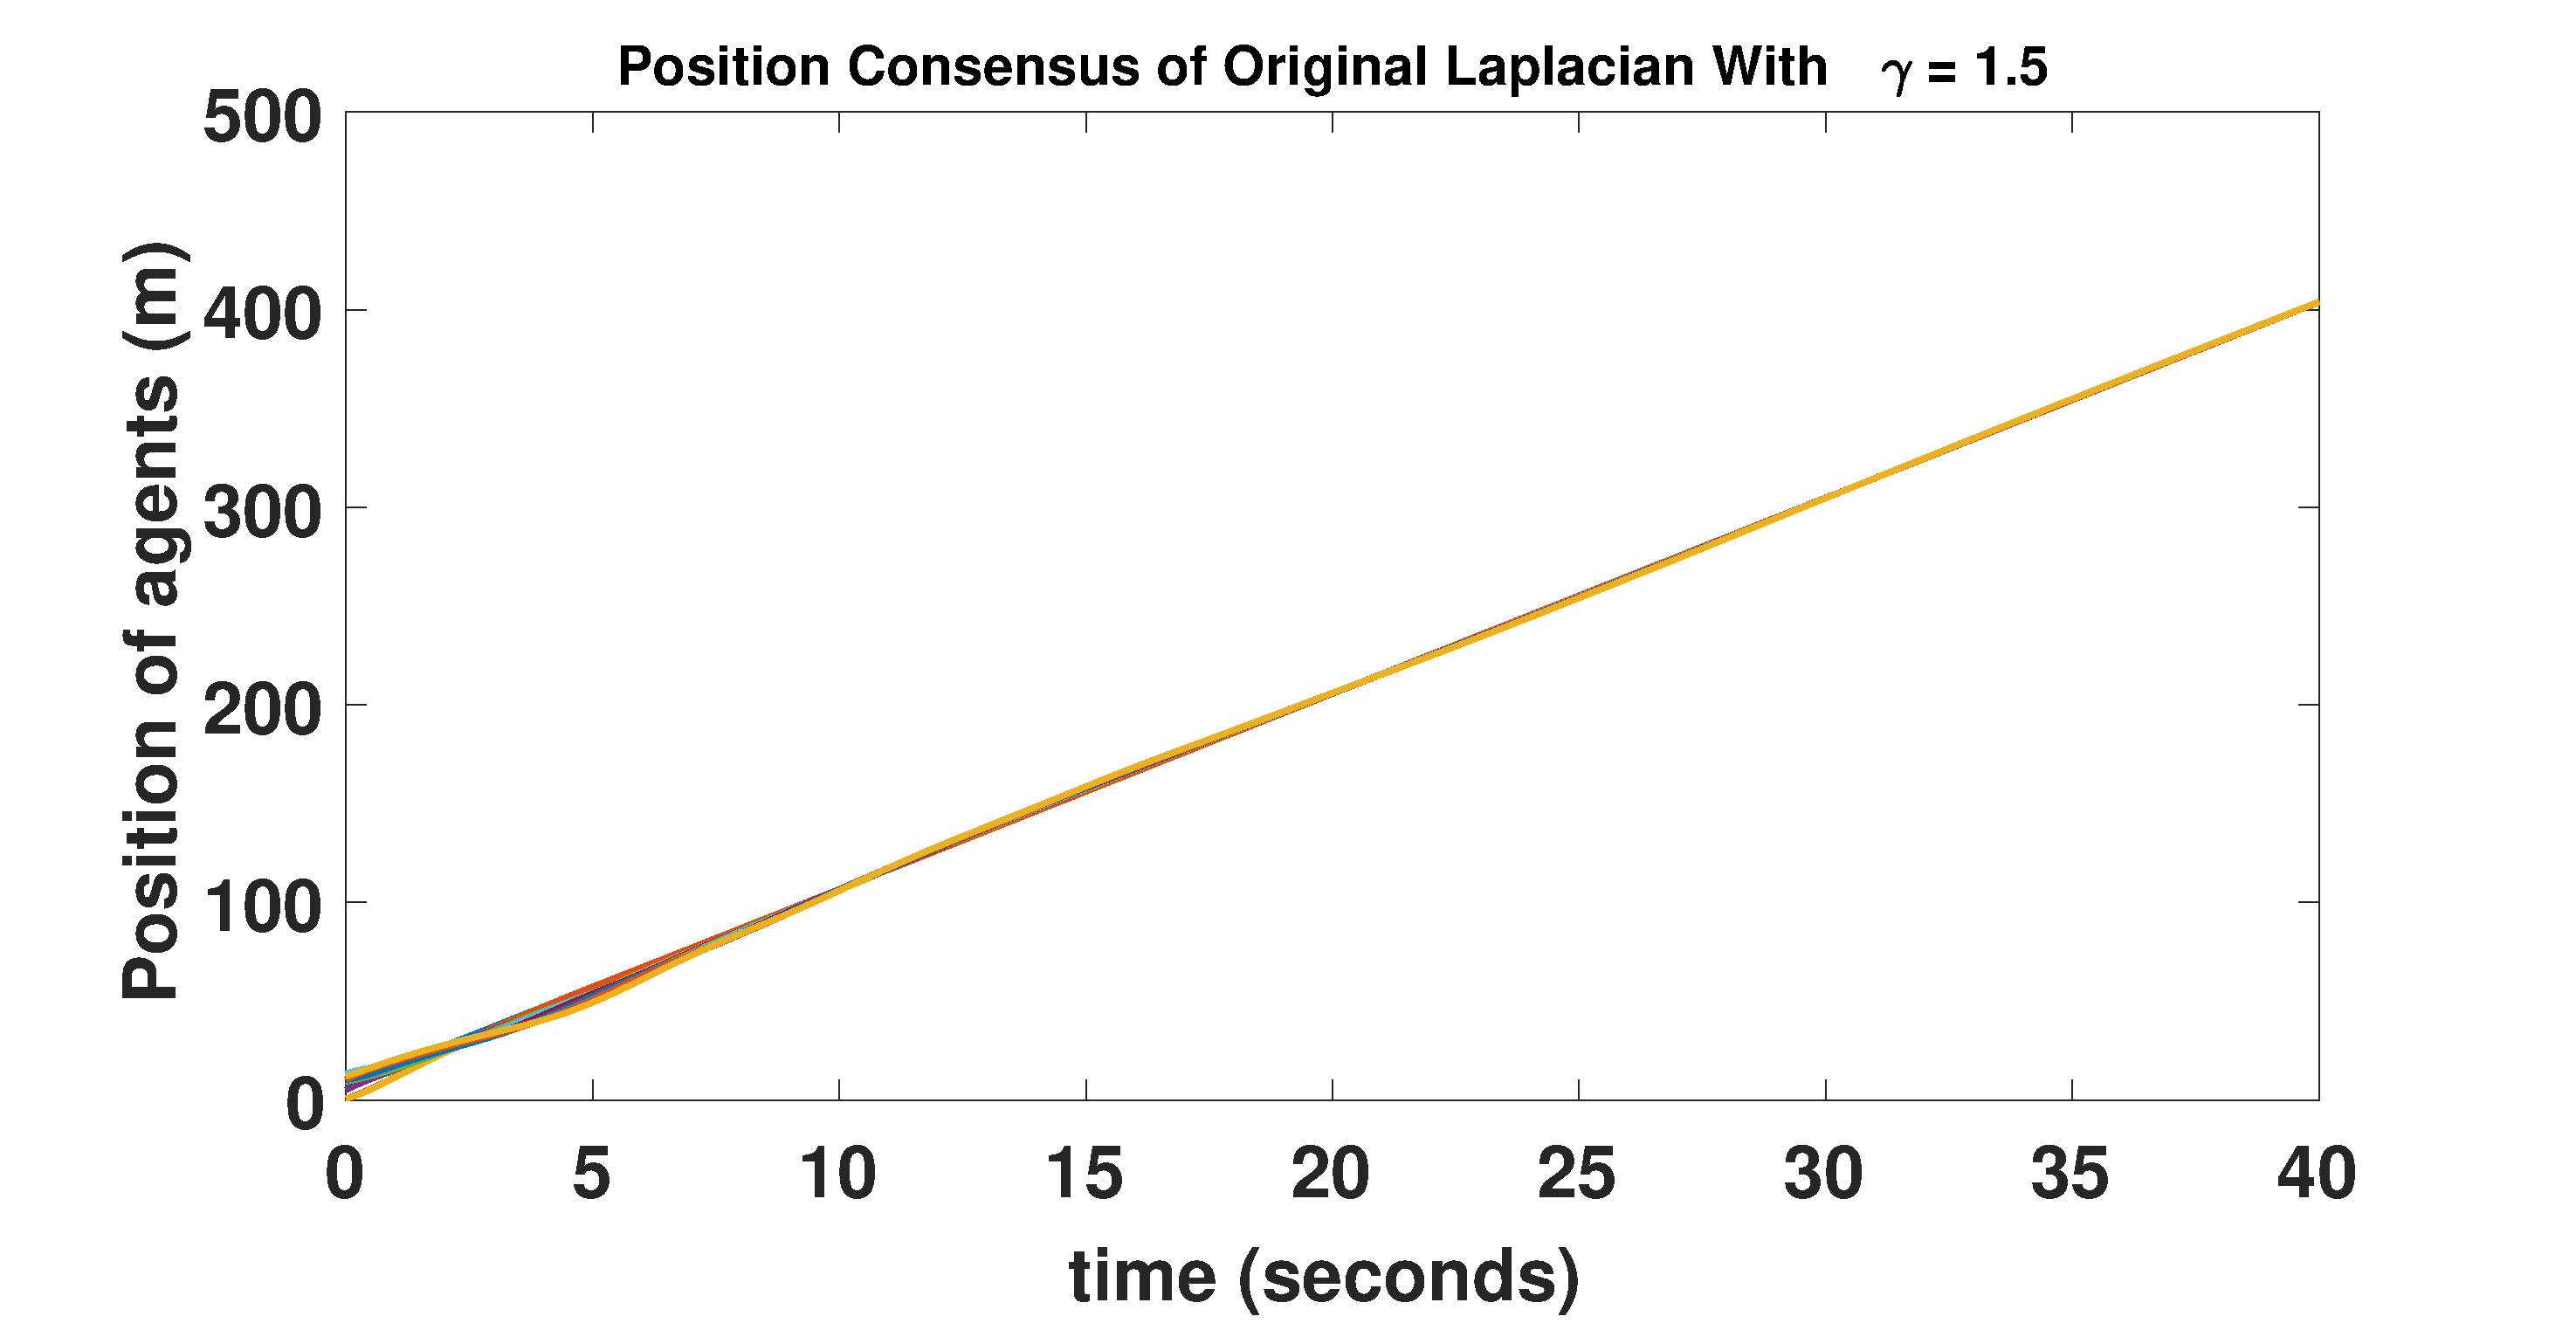
\includegraphics[width=\textwidth, keepaspectratio]{3_Images/10-9-3_OriginalLaplacianGamma1.5PositionConsensus.eps}
		\caption{Position consensus restored ($\gamma = 1.5$).}
		\label{fig:10-9-3_OriginalLaplacianGamma1.5PositionConsensus}
	\end{subfigure}
	\hfill
	\begin{subfigure}[b]{\textwidth}
		\centering
		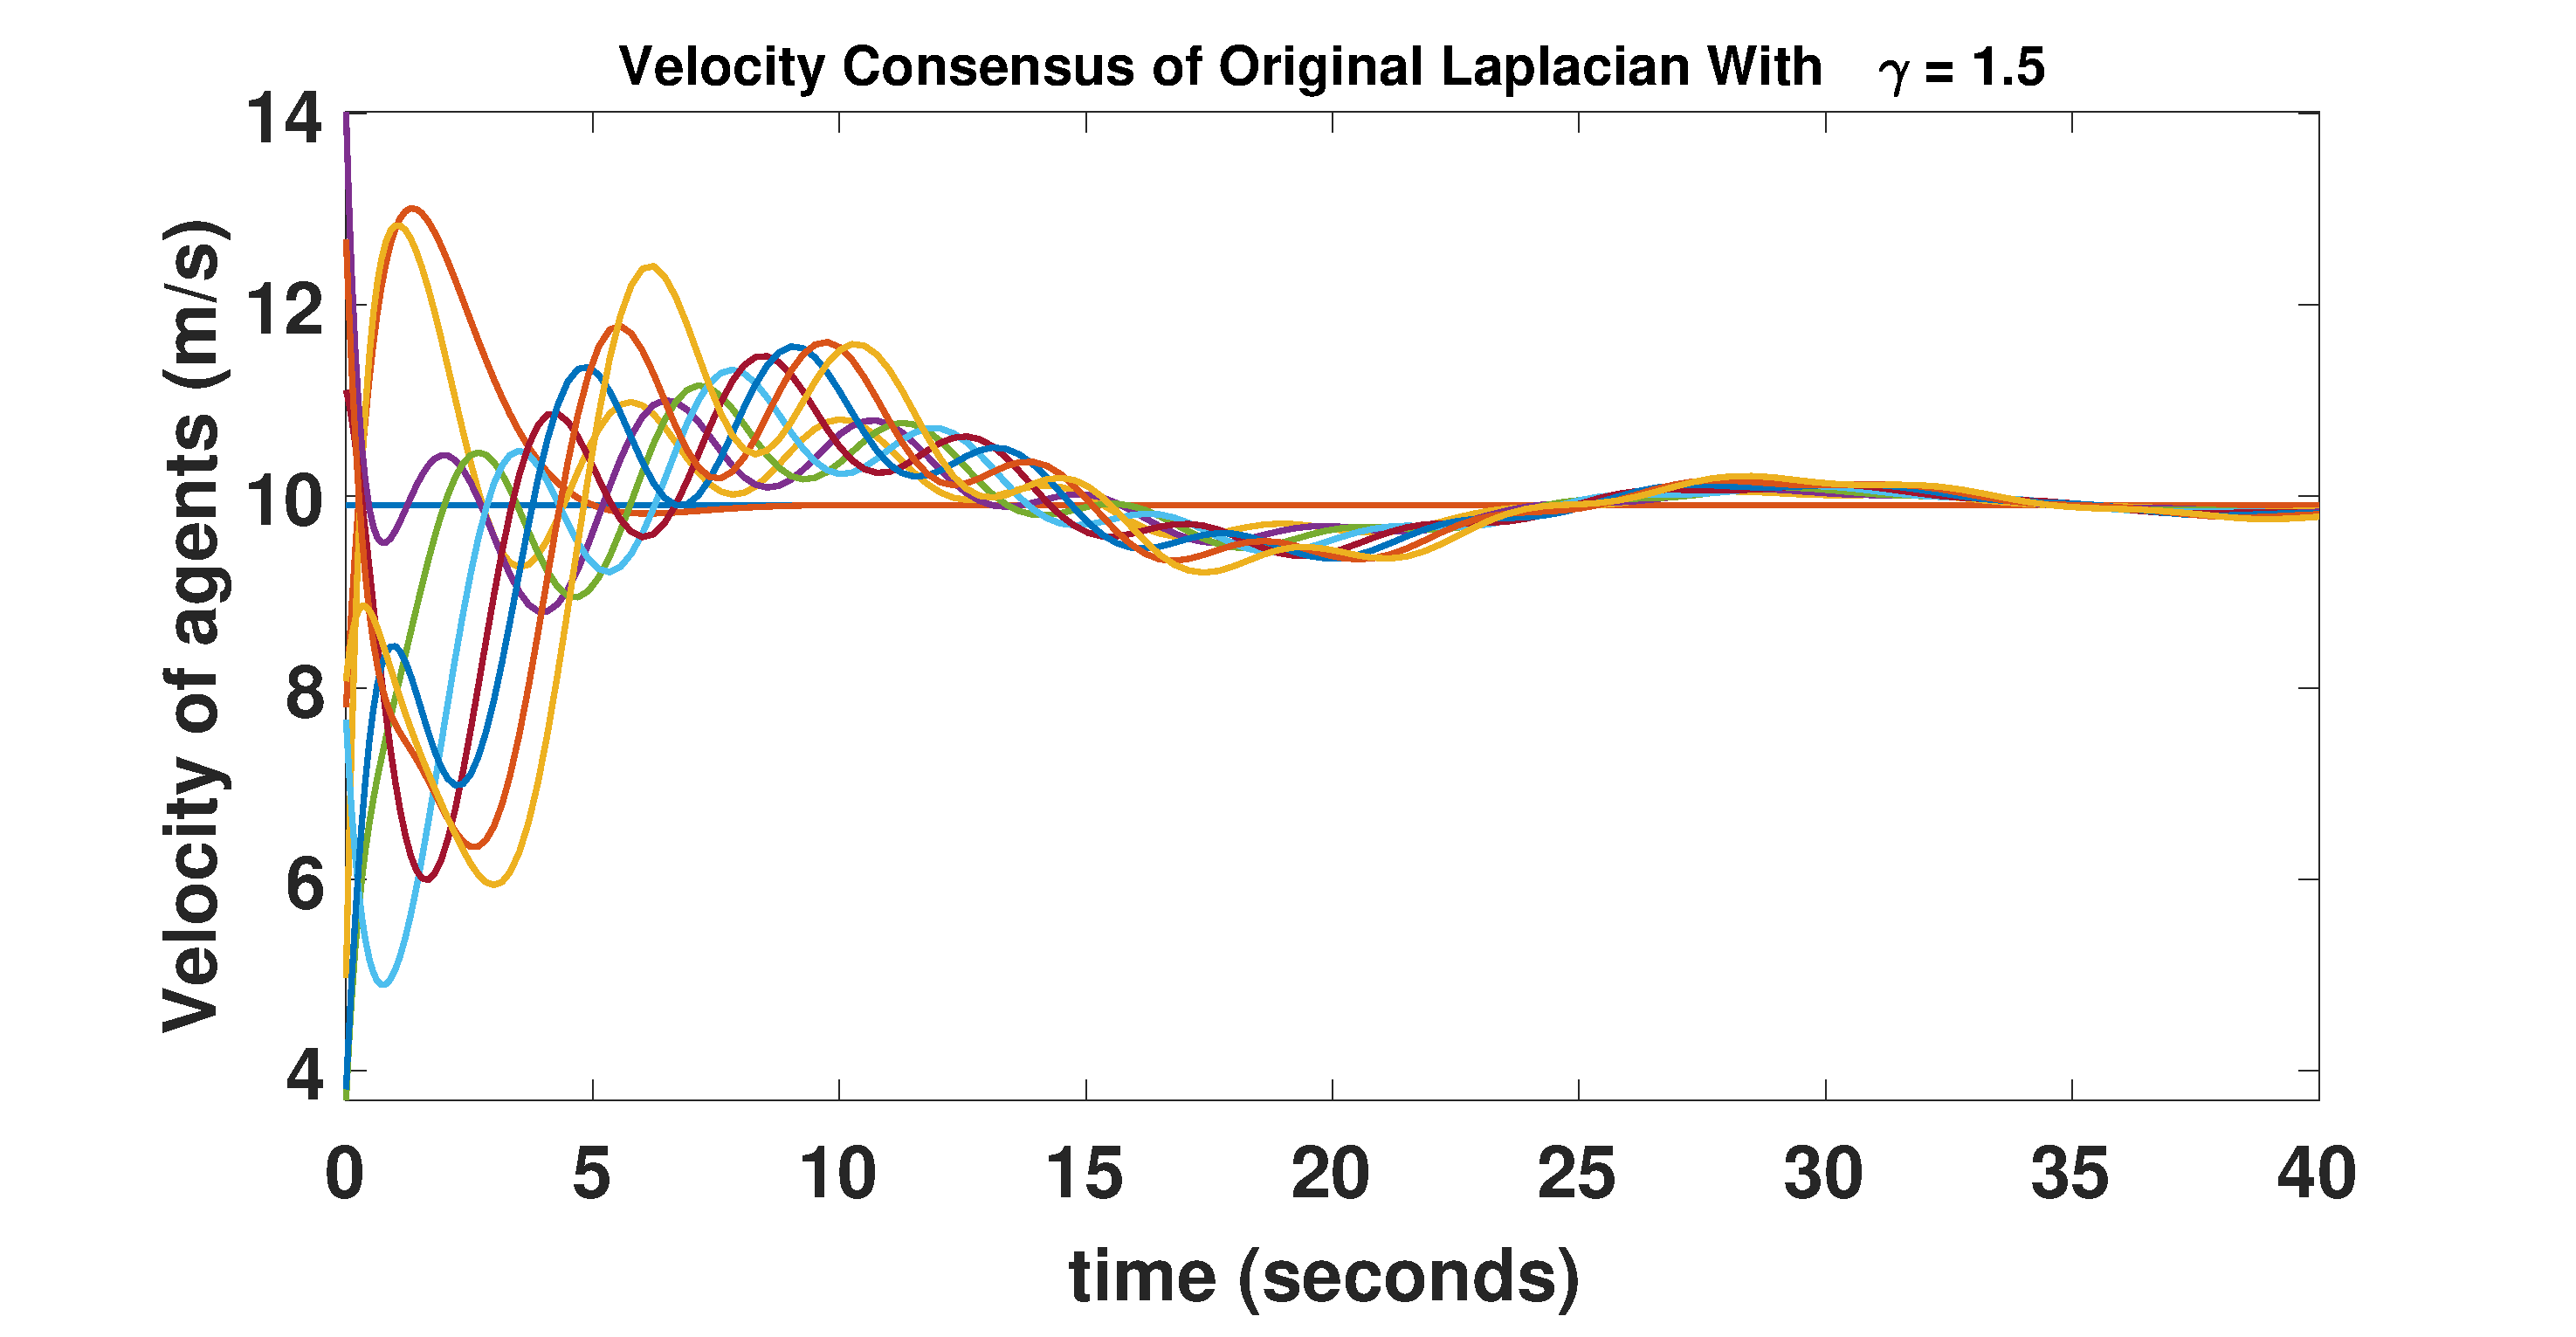
\includegraphics[width=\textwidth, keepaspectratio]{3_Images/10-9-3_OriginalLaplacianGamma1.5VelocityConsensus.eps}
		\caption{Velocity consensus restored ($\gamma = 1.5$).}
		\label{fig:10-9-3_OriginalLaplacianGamma1.5VelocityConsensus}
	\end{subfigure}
	\caption{Restoration of consensus by retuning global coupling to $\gamma = 1.5 > 1.2134$ (requires global network access).}
	\label{fig:global_retuning}
\end{figure}
\subsection{Validation of Localized Scaling Remedies ($x_1 = 3 > 1$)}
We now apply the localized scaling remedies without modifying $\gamma = 0.5$:

1. \textbf{Node-Based Scaling:} Applying Theorem \ref{theo1} with $\gamma = 0.5$ and $\ell = 6$, $p_1 \ge \frac{7}{0.25} = 28$. Selecting $p_1 = 31.5$ and creating a 7-term AP between $p_1 = 31.5$ and $2p_1 = 63$ gives common difference $d = 4.5$. The scaling matrix is $P = \text{diag}(31.5, 58.5, 54, 49.5, 45, 40.5, 36)$. Under $P$, the required coupling threshold drops to $\gamma \ge 0.1822 < 0.5$. Figures \ref{fig:10-9-3_NodeScaledLaplacianGamma0.5PositionConsensus} and \ref{fig:10-9-3_NodeScaledLaplacianGamma0.5VelocityConsensus} confirm asymptotic state agreement under $\gamma = 0.5$.

\begin{figure}[ht!]
	\centering
	\begin{subfigure}[b]{\textwidth}
		\centering
		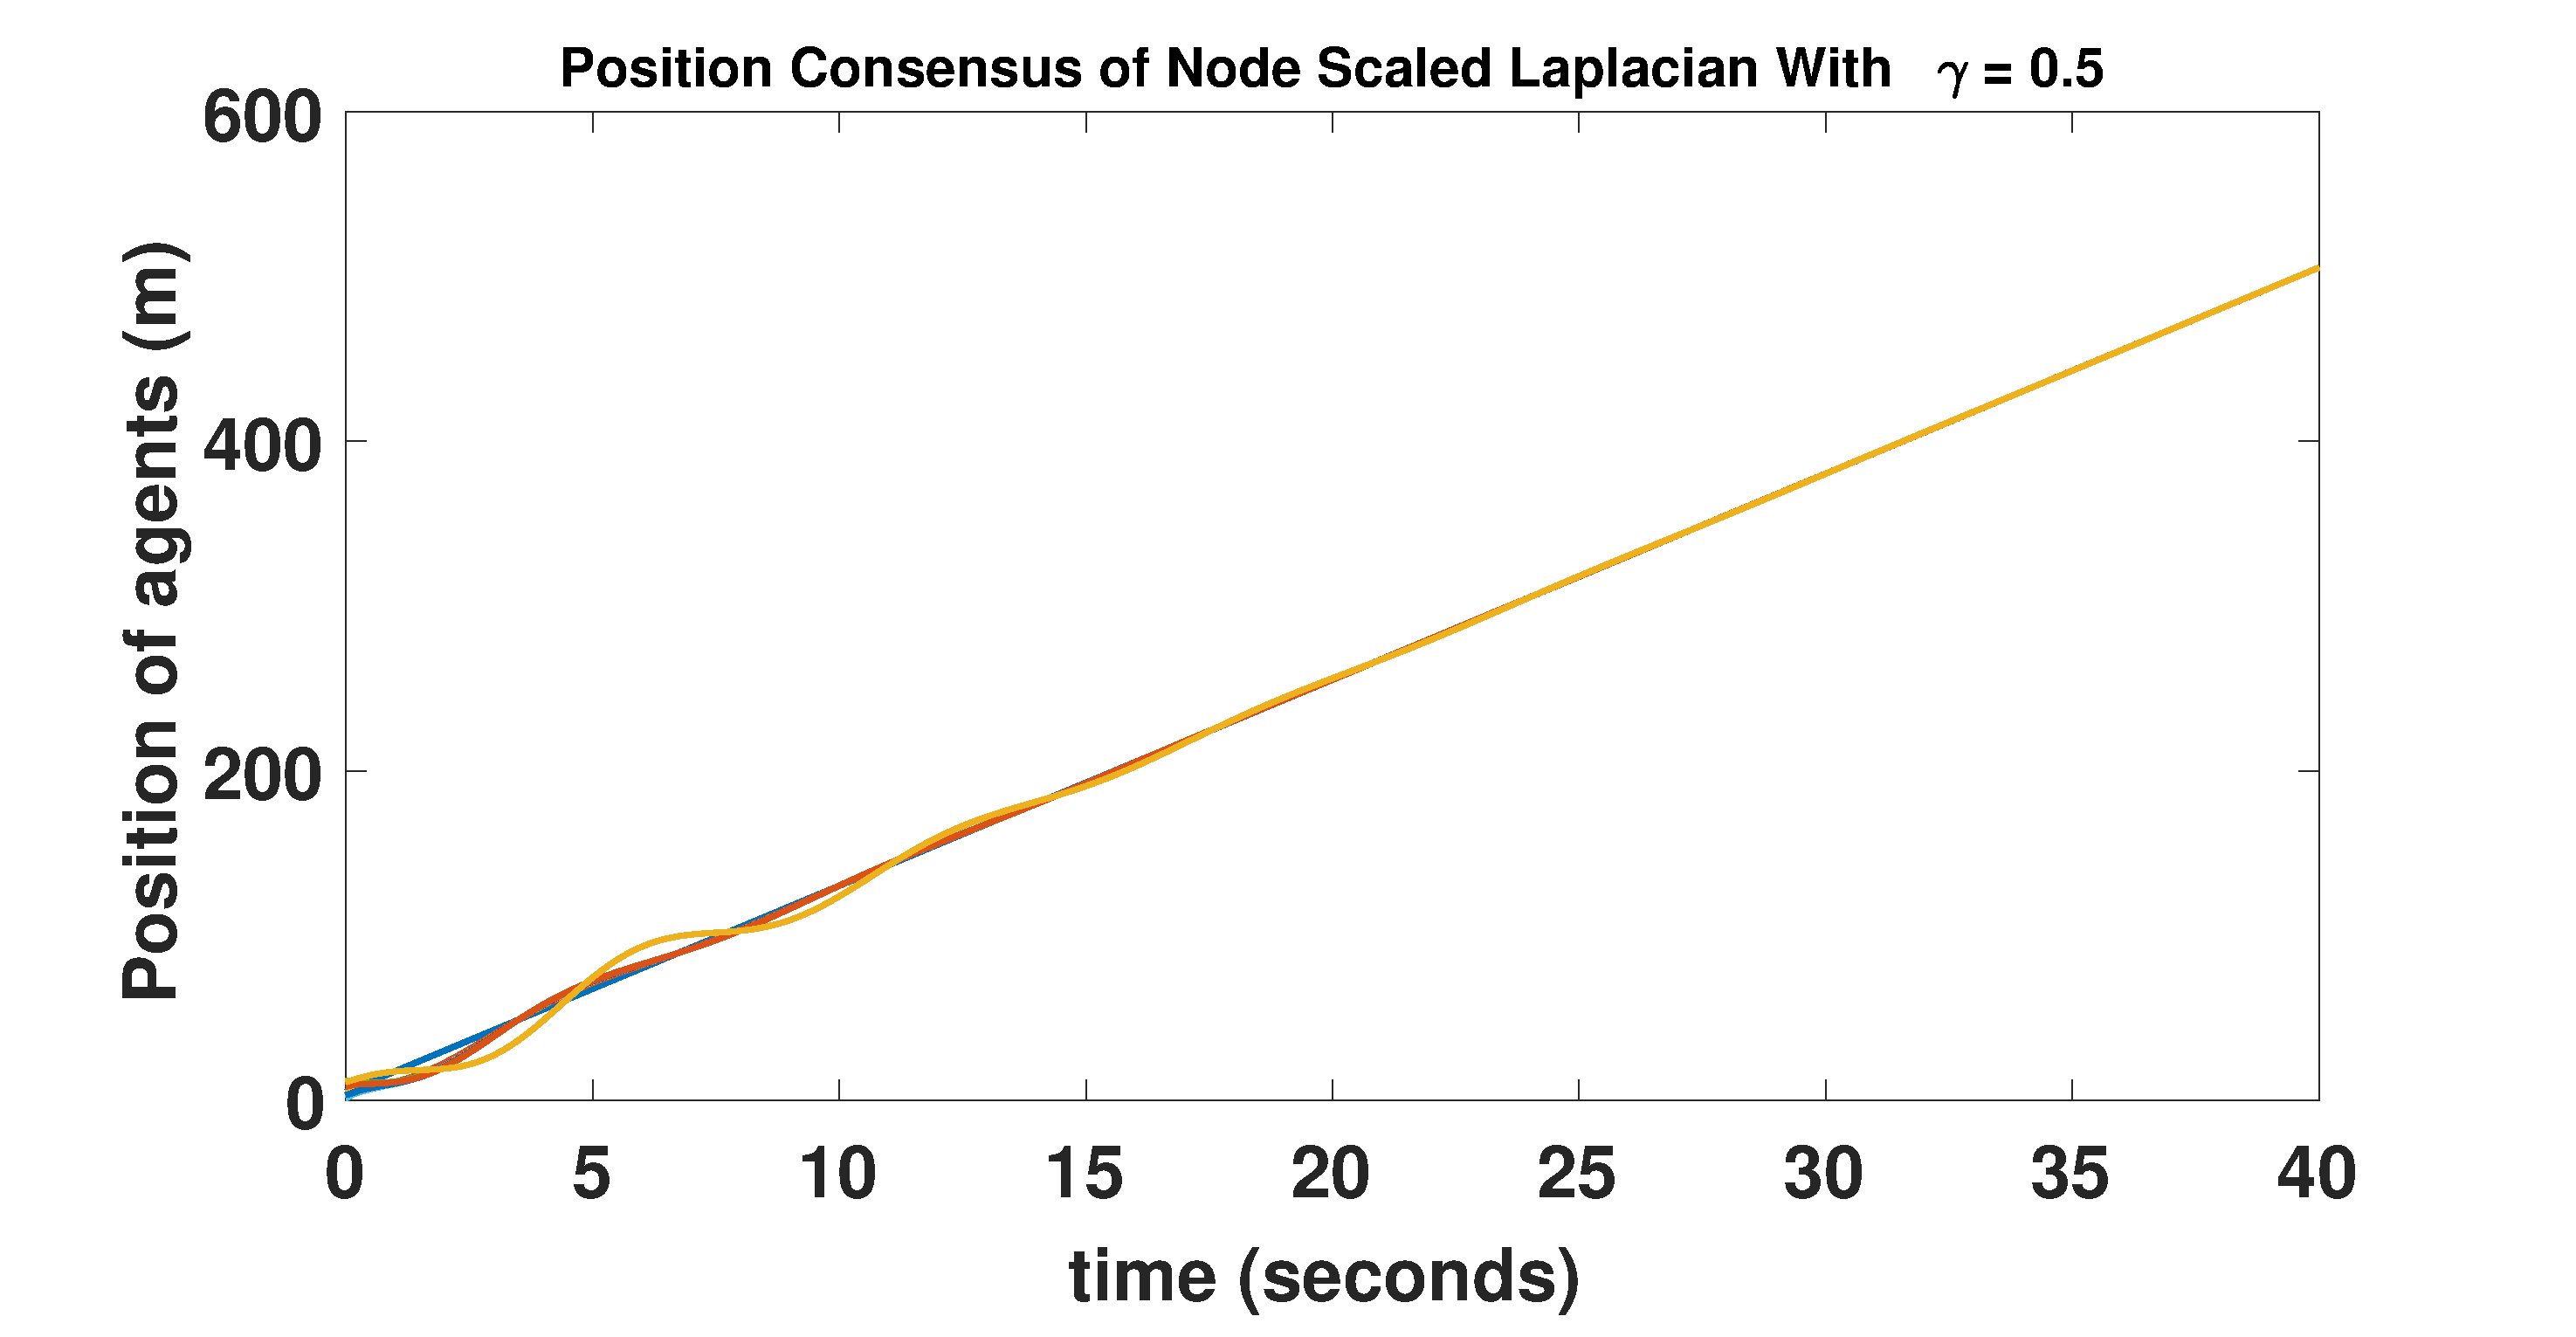
\includegraphics[width=\textwidth, keepaspectratio]{3_Images/10-9-3_NodeScaledLaplacianGamma0.5PositionConsensus.eps}
		\caption{Node-Scaled Position Consensus ($\gamma = 0.5$).}
		\label{fig:10-9-3_NodeScaledLaplacianGamma0.5PositionConsensus}
	\end{subfigure}
	\hfill
	\begin{subfigure}[b]{\textwidth}
		\centering
		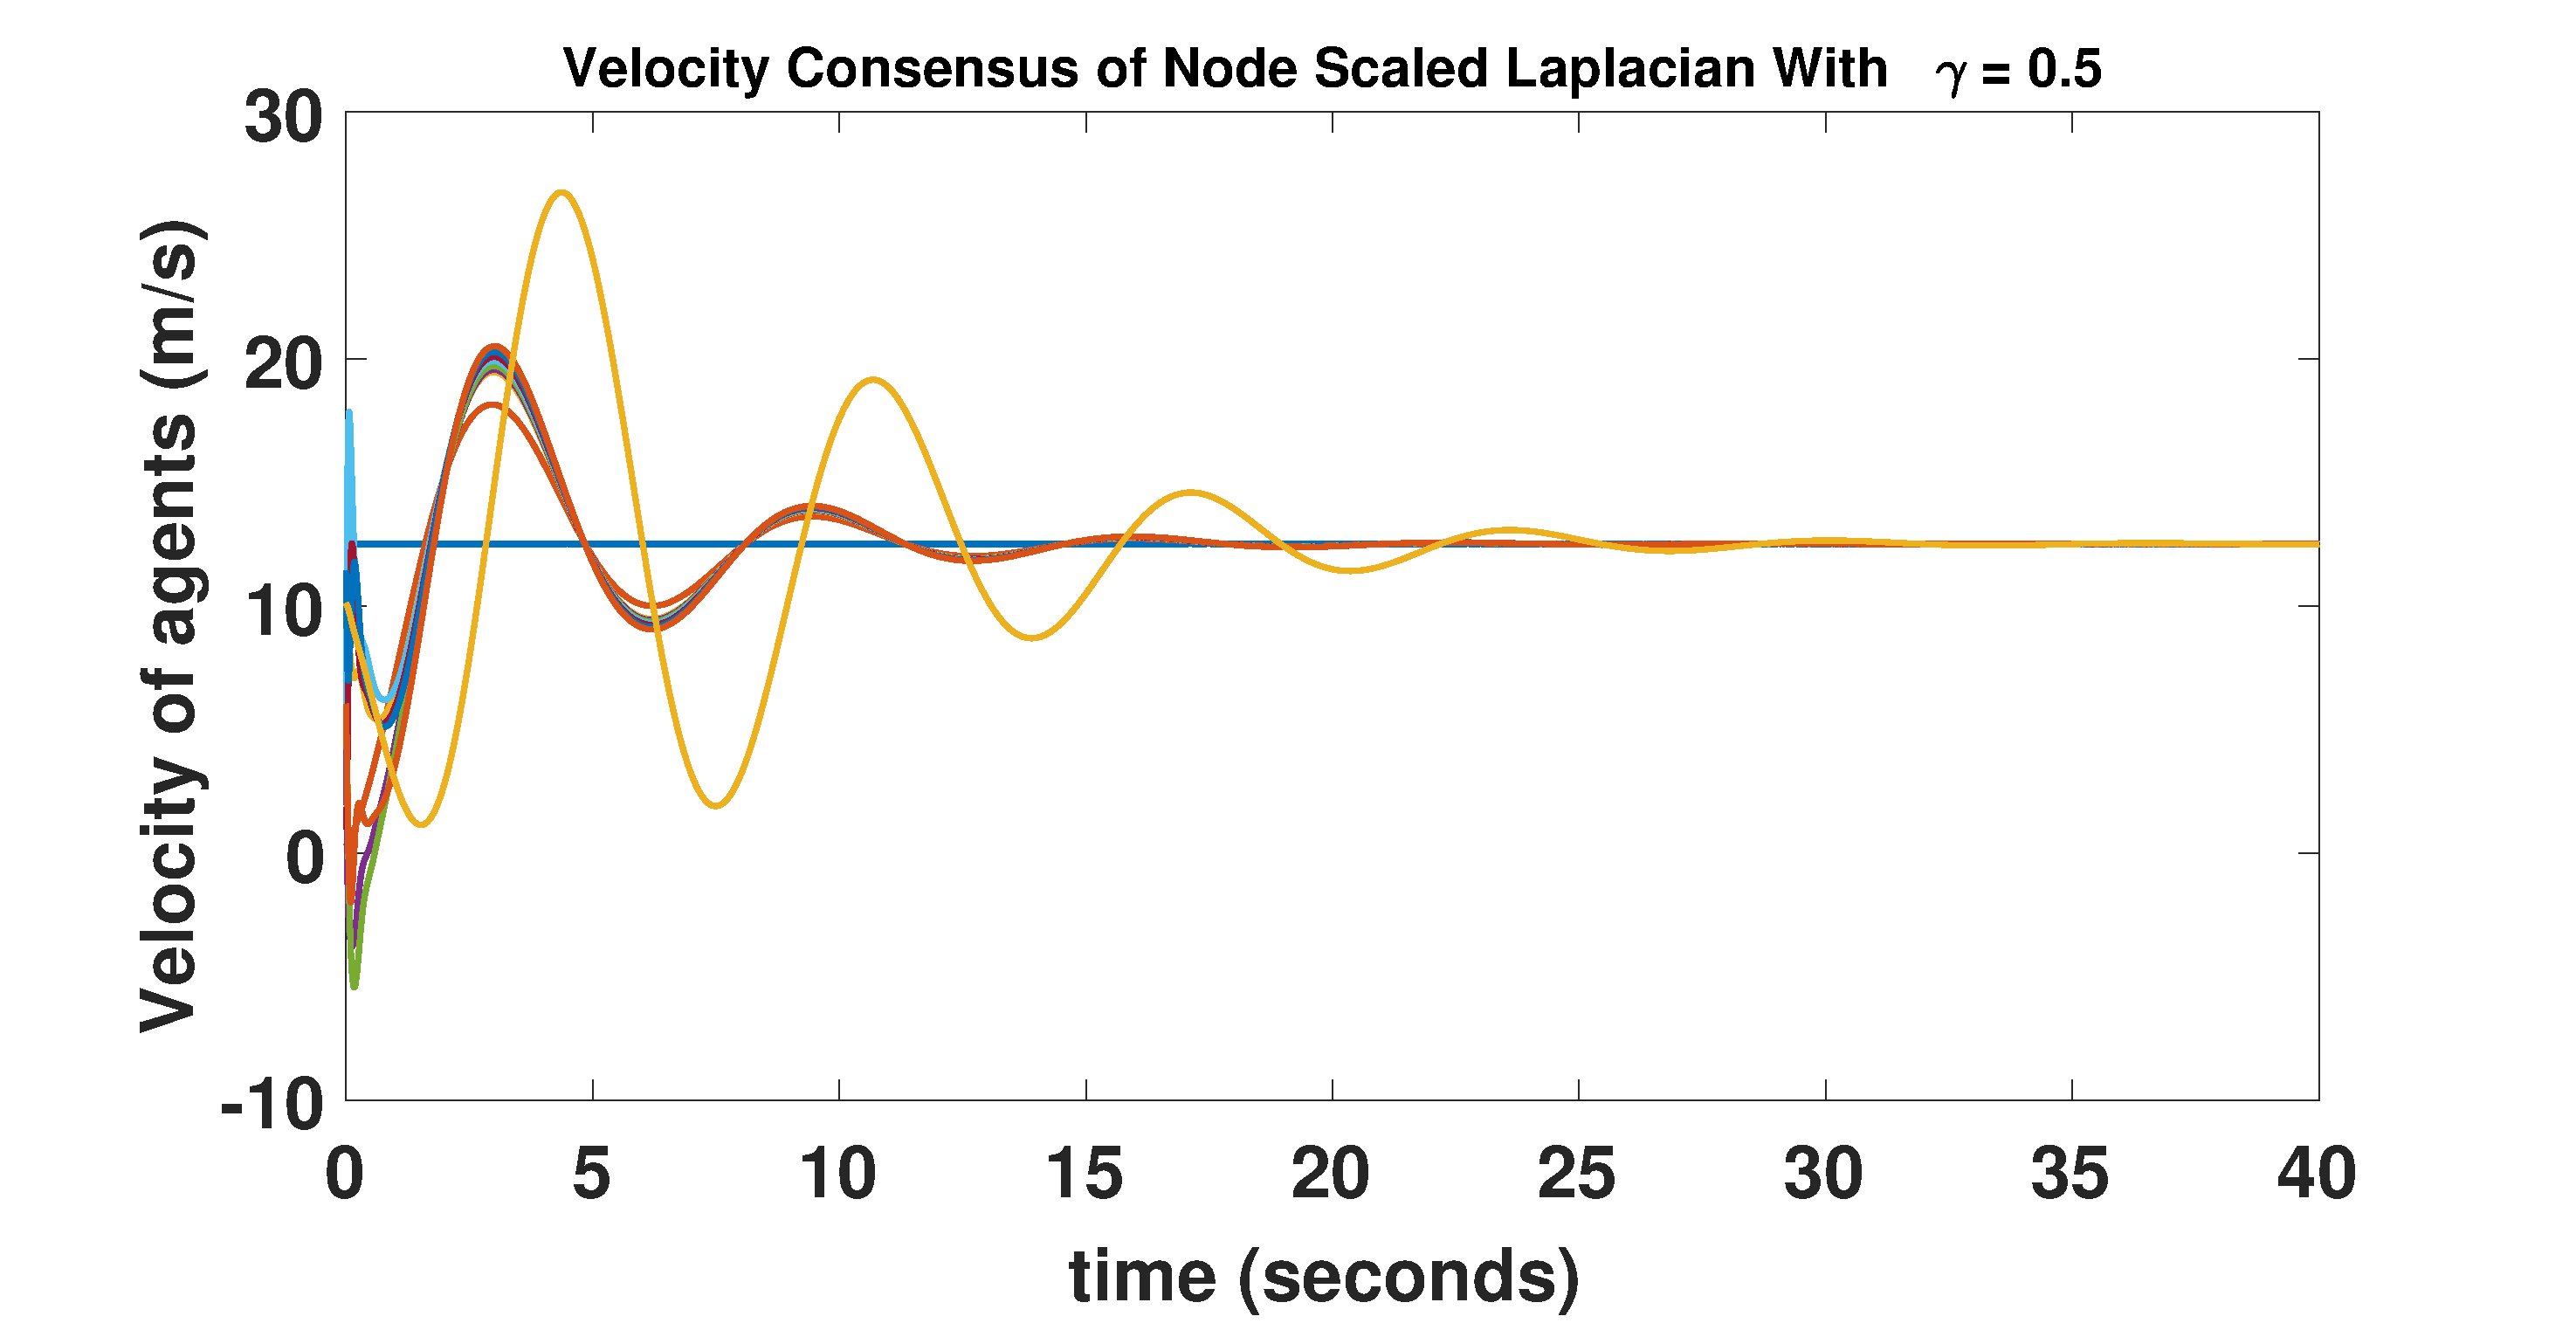
\includegraphics[width=\textwidth, keepaspectratio]{3_Images/10-9-3_NodeScaledLaplacianGamma0.5VelocityConsensus.eps}
		\caption{Node-Scaled Velocity Consensus ($\gamma = 0.5$).}
		\label{fig:10-9-3_NodeScaledLaplacianGamma0.5VelocityConsensus}
	\end{subfigure}
	\caption{Consensus restored using Node-Based Scaling ($p_1 = 31.5, d = 4.5$) under fixed global parameter $\gamma = 0.5$.}
	\label{fig:NodeScaling_sims}
\end{figure}

2. \textbf{Edge-Based Scaling:} Applying Theorem \ref{theo2} with $w_r = 1$, $w_1 \ge 28$. Selecting $w_1 = 31.5$, an AP between $w_1 + w_r = 32.5$ and $w_r = 1$ gives $d = 4.5$, yielding edge weights $\{31.5, 28, 23.5, 19, 14.5, 10, 5.5\}$. The required threshold drops to $\gamma \ge 0.1245 < 0.5$. Figures \ref{fig:10-9-3_ReverseEdgeScaledLaplacianGamma0.5PositionConsensus} and \ref{fig:10-9-3_ReverseEdgeScaledLaplacianGamma0.5VelocityConsensus} demonstrate smooth state convergence.

\begin{figure}[ht!]
	\centering
	\begin{subfigure}[b]{\textwidth}
		\centering
		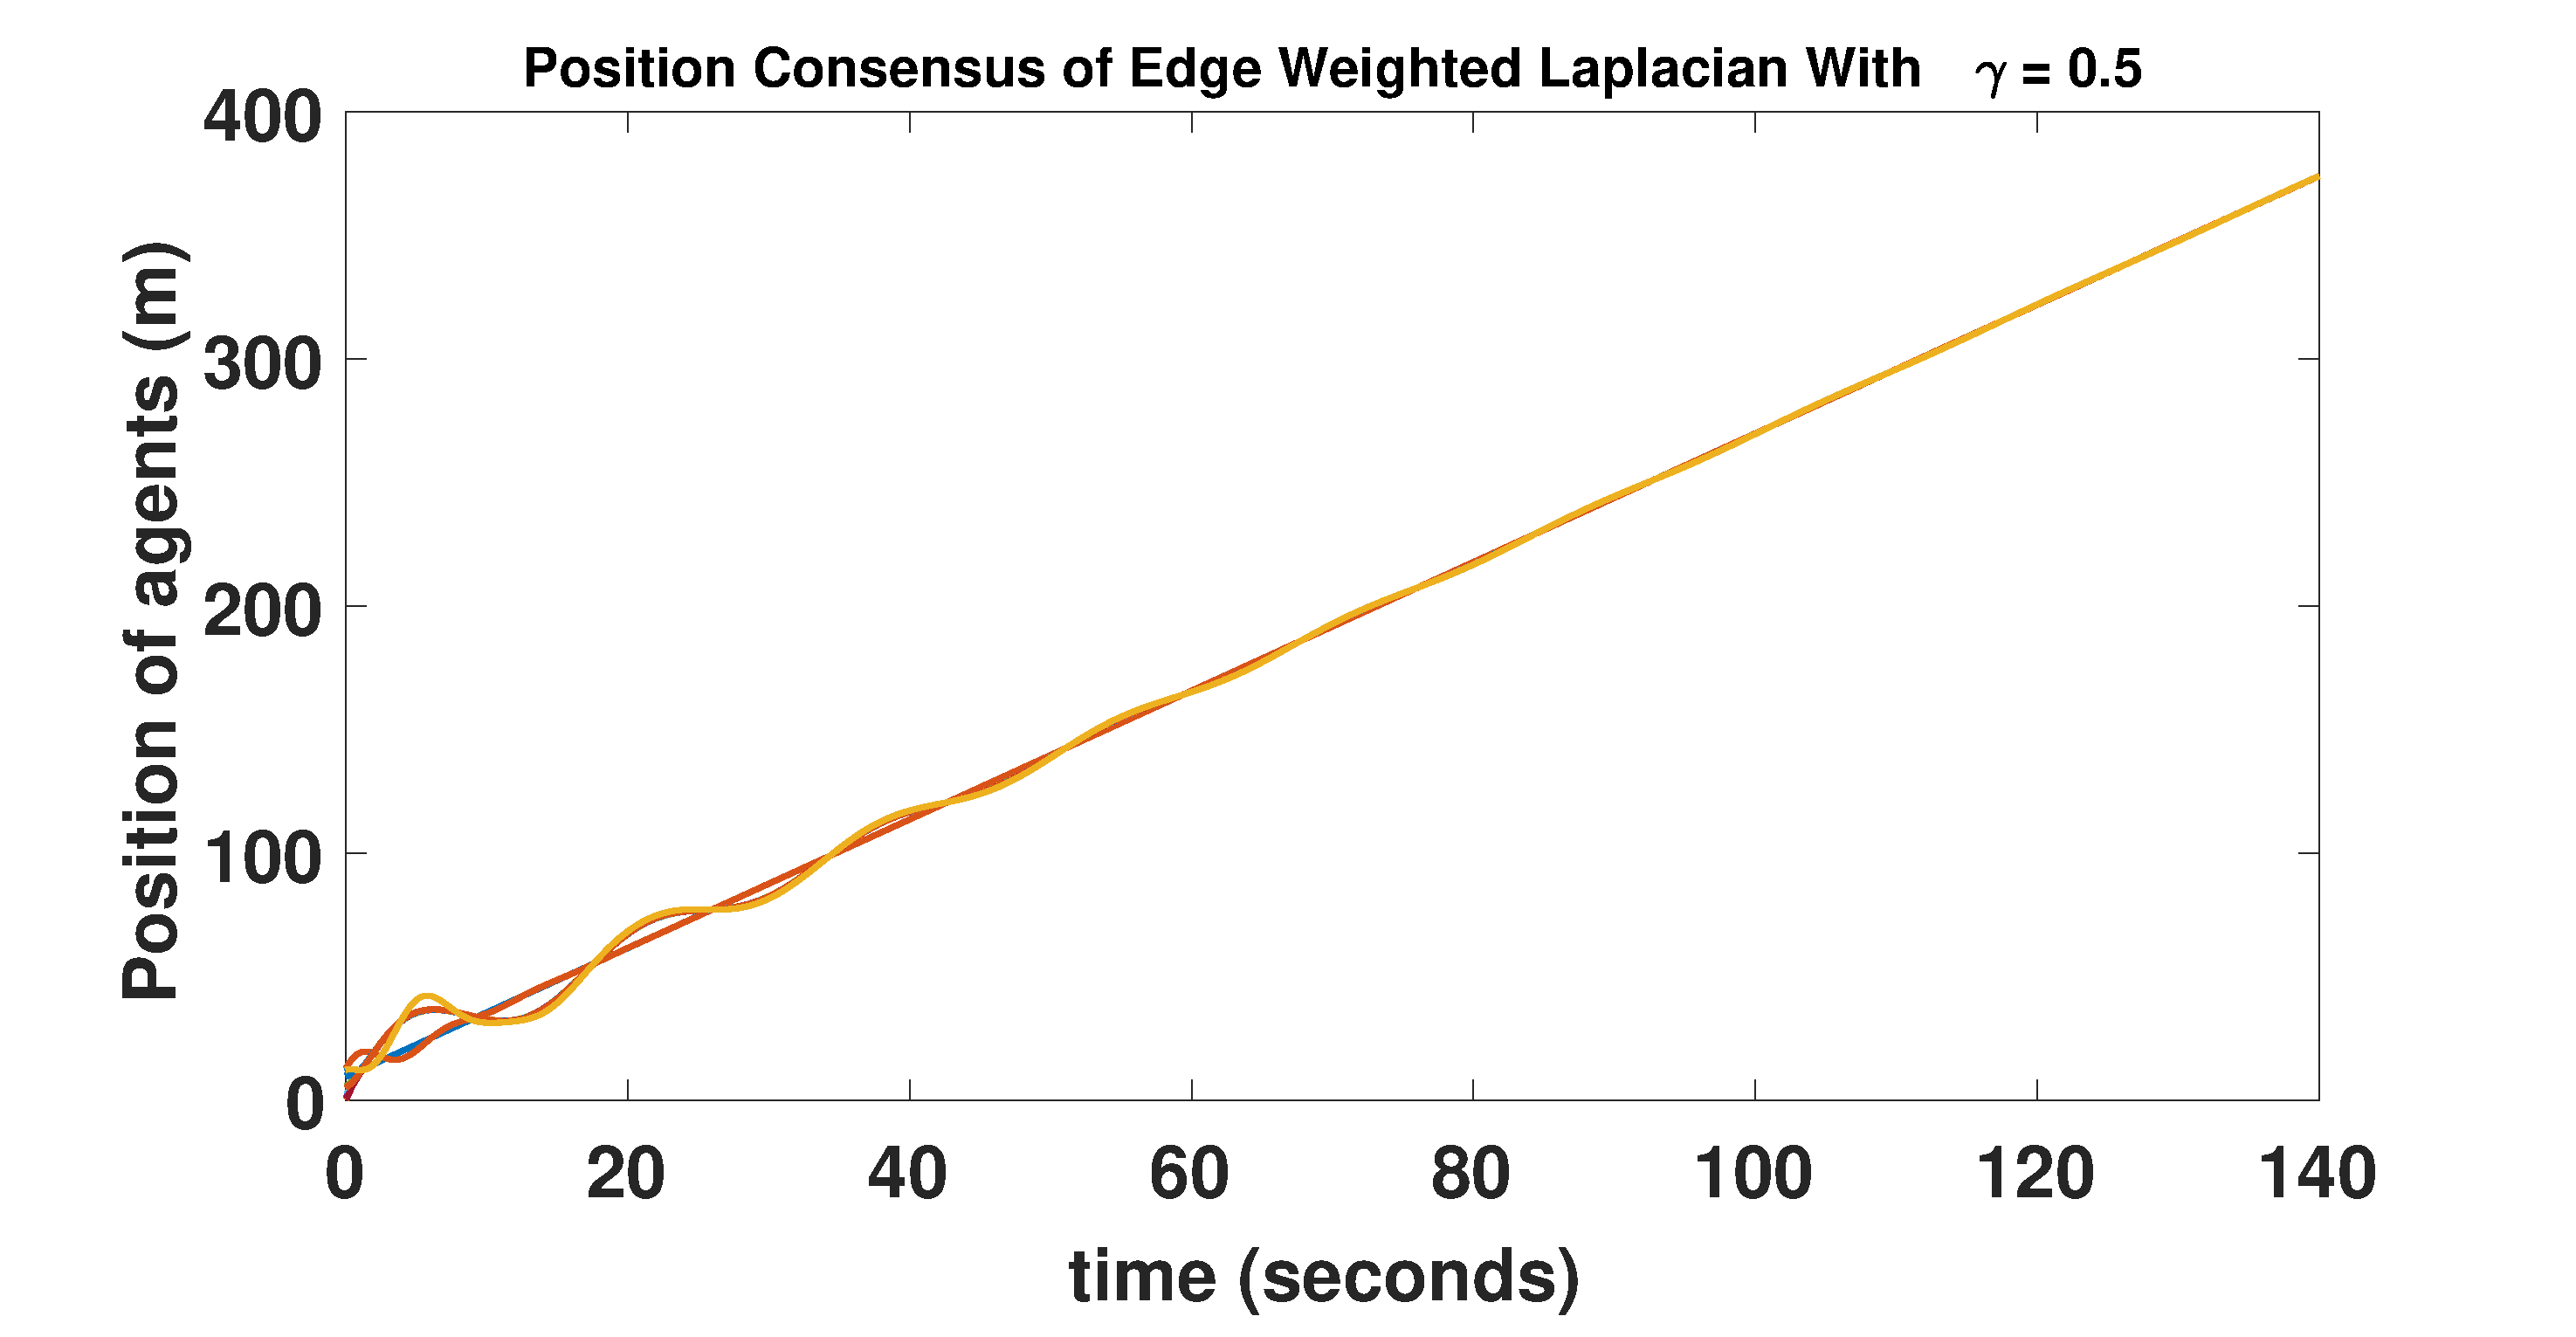
\includegraphics[width=\textwidth, keepaspectratio]{3_Images/10-9-3_ReverseEdgeScaledLaplacianGamma0.5PositionConsensus.eps}
		\caption{Edge-Scaled Position Consensus.}
		\label{fig:10-9-3_ReverseEdgeScaledLaplacianGamma0.5PositionConsensus}
	\end{subfigure}
	\hfill
	\begin{subfigure}[b]{\textwidth}
		\centering
		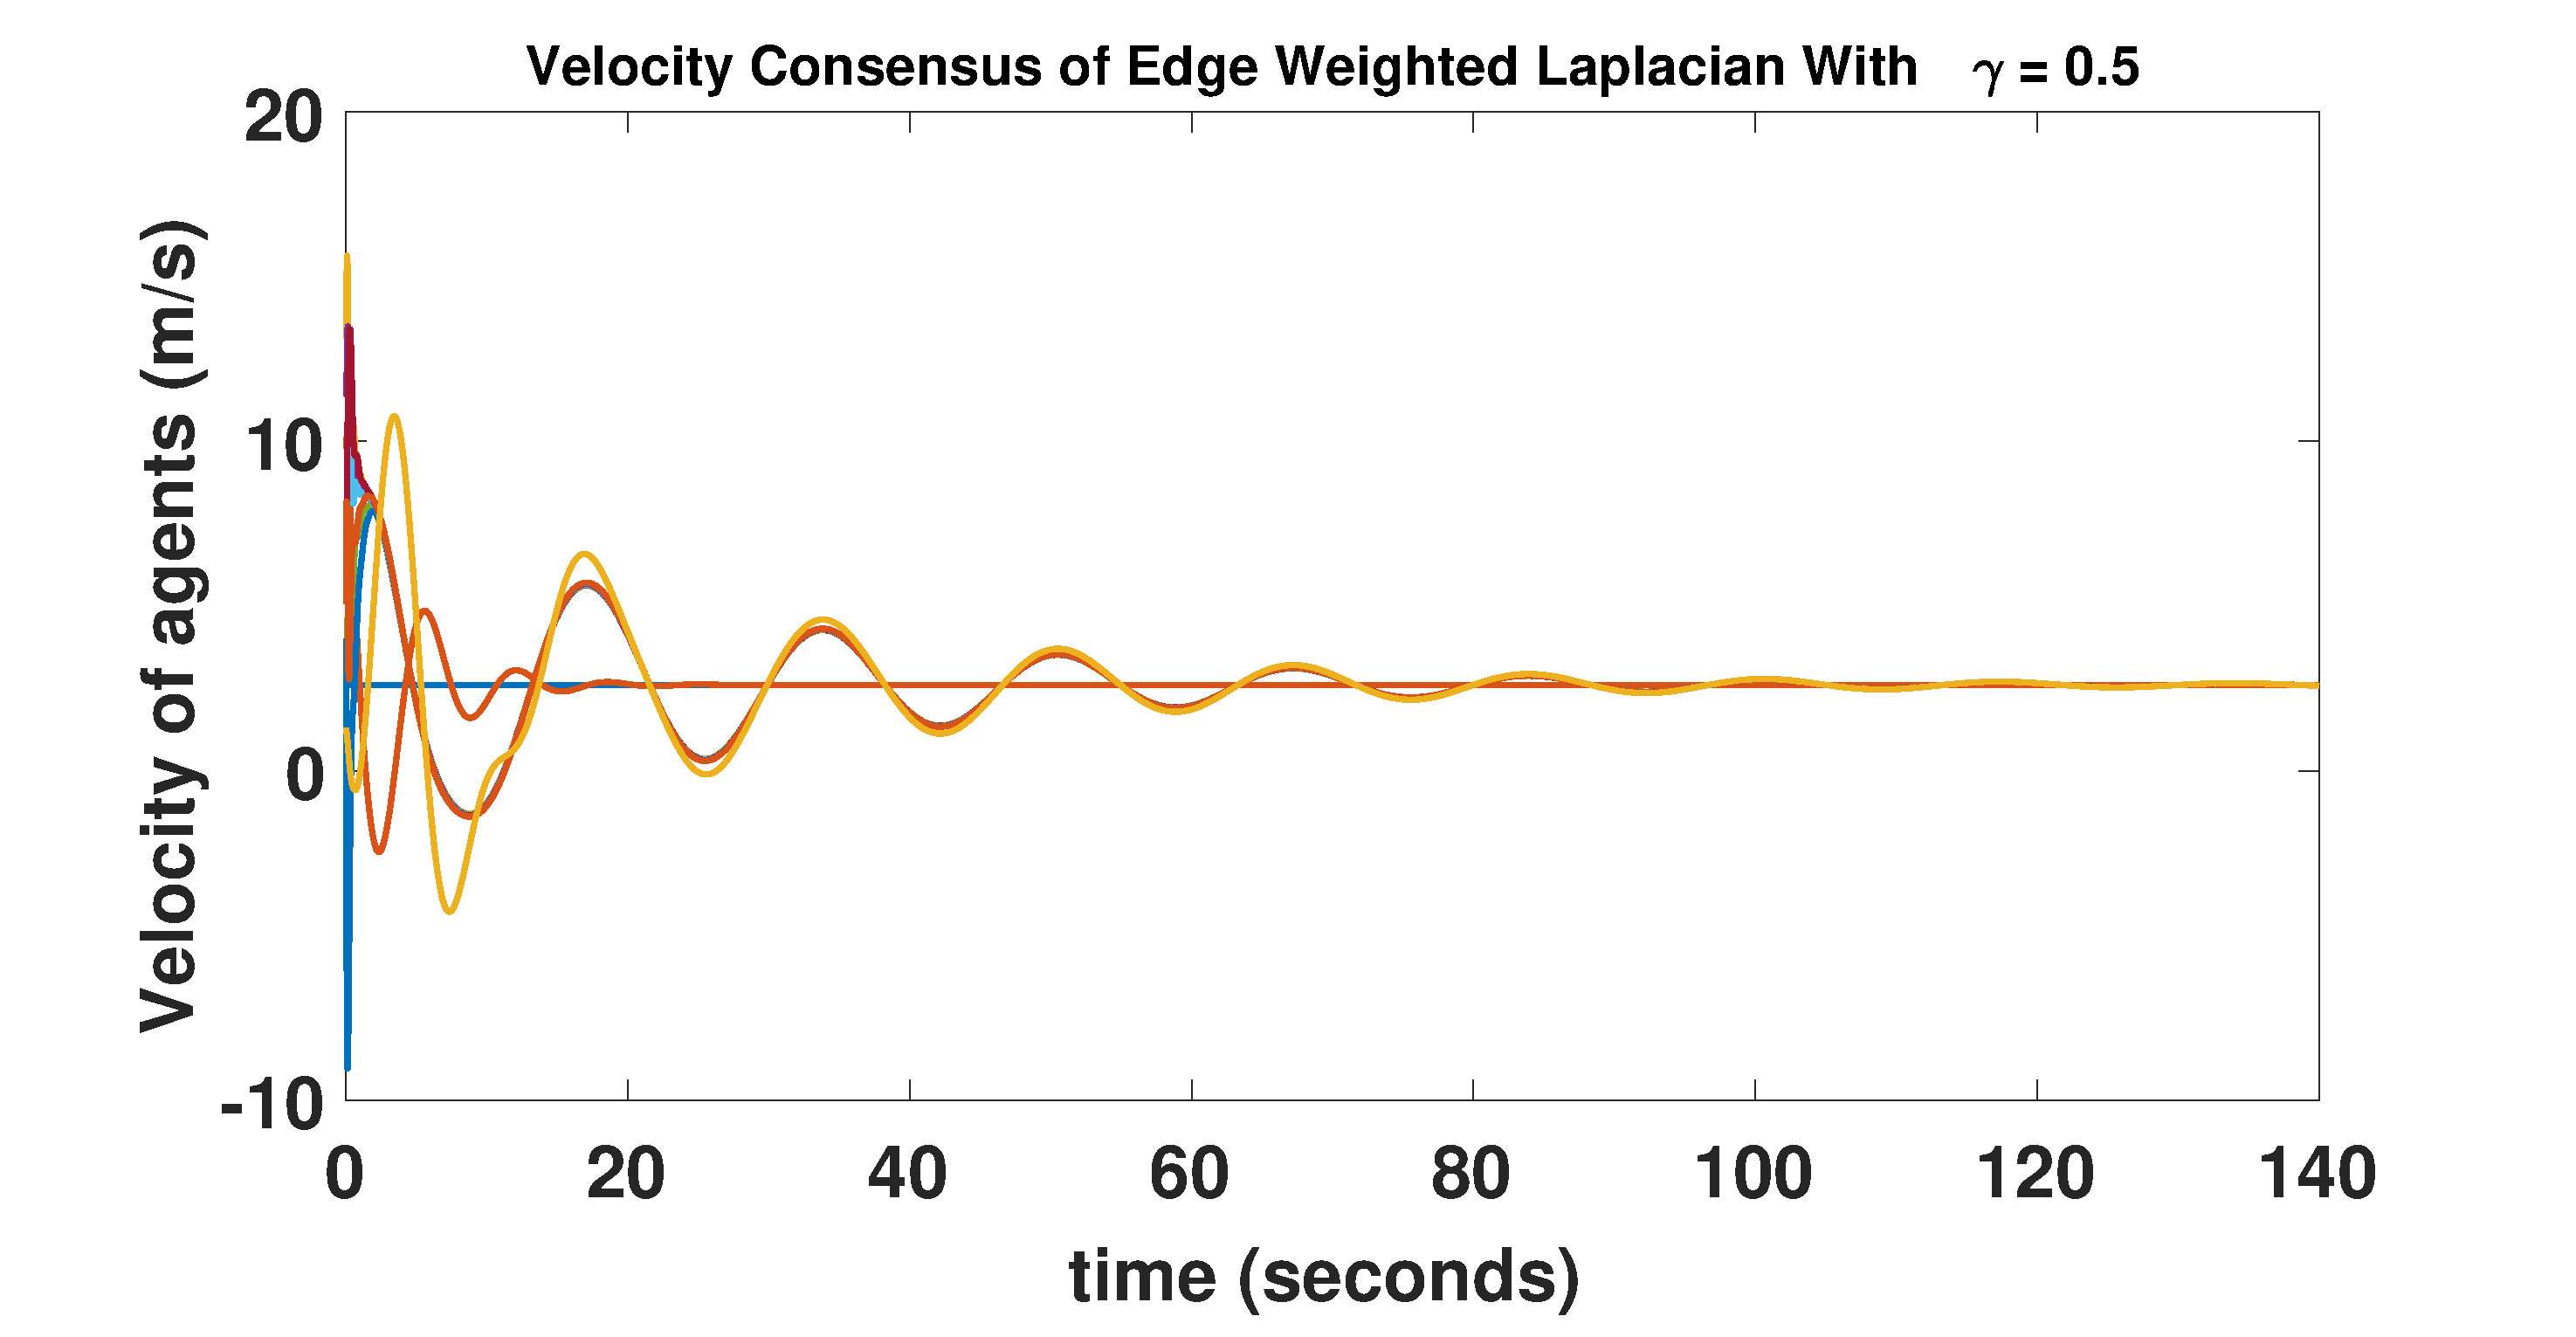
\includegraphics[width=\textwidth, keepaspectratio]{3_Images/10-9-3_ReverseEdgeScaledLaplacianGamma0.5VelocityConsensus.eps}
		\caption{Edge-Scaled Velocity Consensus.}
		\label{fig:10-9-3_ReverseEdgeScaledLaplacianGamma0.5VelocityConsensus}
	\end{subfigure}
	\caption{Consensus restored using Edge-Based Scaling ($w_1 = 31.5, d = 4.5$) under fixed global parameter $\gamma = 0.5$.}
	\label{fig:EdgeScaling_sims}
\end{figure}

3. \textbf{Combined Scaling:} Setting $w_1 = 1$ and $p_1 = 31.5$, edge weights are tuned within the practical hardware range $w_k \in [1, 2]$ ($w_7 = 1.8571, w_6 = 1.7143, w_5 = 1.5714, w_4 = 1.4286, w_3 = 1.2857, w_2 = 1.1429$). The required threshold drops to $\gamma \ge 0.1164 < 0.5$, confirming practical realizability.

\subsection{Validation of Root-Locus Method for Cycle involving the Root Node ($x_1 = 1$)}
Consider a 10-agent network where the reverse edge enters Node 1 ($x_1 = 1, y_1 = 7, \ell = 6$). Fixed coupling is $\gamma = 0.5$. By Theorem \ref{theo3ES}, selecting $\alpha = 9 > 1/\gamma^2 = 4$, the complementary root-locus $G(s) = \frac{\beta\{(s-9)^6 - (-9)^6\}}{s(s-9)^6}$ is plotted in Figures \ref{fig:ComplimentaryRootLocus} and \ref{fig:MirroredComplimentaryRootLocus}. 

The gain margin for stability is $0.6503$. Selecting $\beta = 0.6438$ (giving edge weight $w_2 = \beta / \alpha = 0.0715$), the required threshold drops to $\gamma \ge 0.3501$ which is less than 0.5. Figures \ref{fig:NewRootLocusBasedLaplacianPositionConsensus0.5} and \ref{fig:NewRootLocusBasedLaplacianVelocityConsensus0.5} confirm that second-order consensus is successfully achieved under a root-node loop.

\begin{figure}[ht!]
	\centering
	\begin{subfigure}[b]{\textwidth}
		\centering
		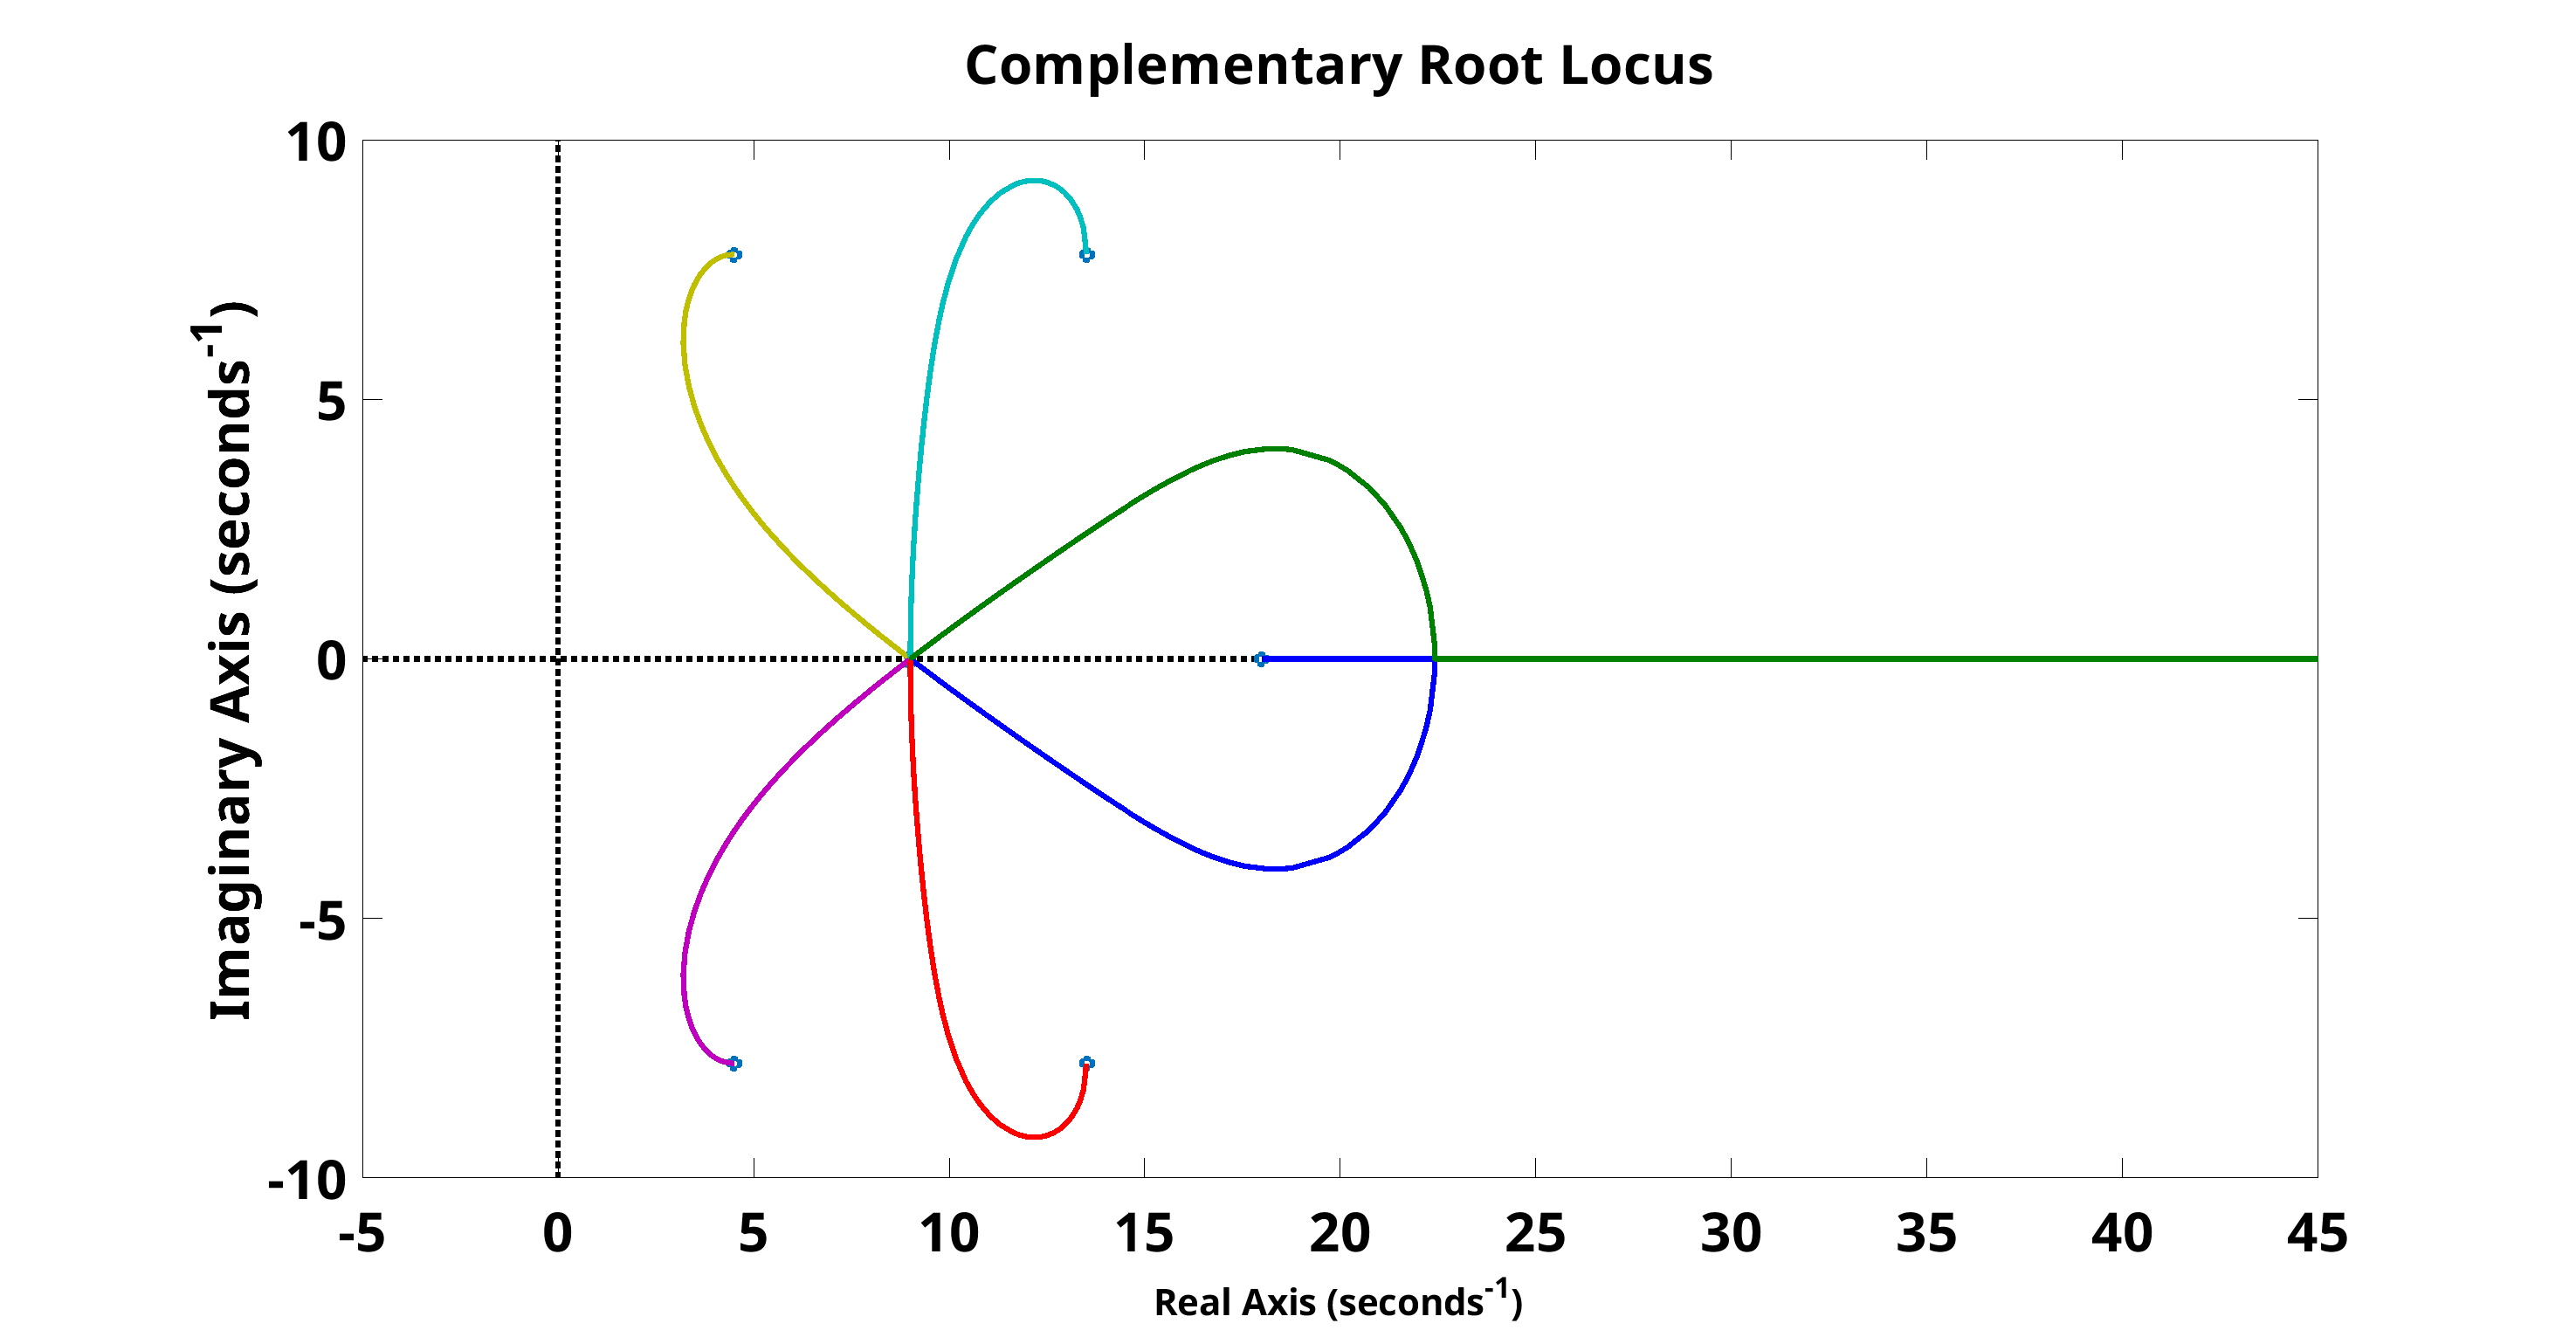
\includegraphics[width=\textwidth, keepaspectratio]{3_Images/CRLwithalpha9.eps}
		\caption{Complementary Root Locus of $G(s)$ for $\alpha = 9$.}
		\label{fig:ComplimentaryRootLocus}
	\end{subfigure}
	\hfill
	\begin{subfigure}[b]{\textwidth}
		\centering
		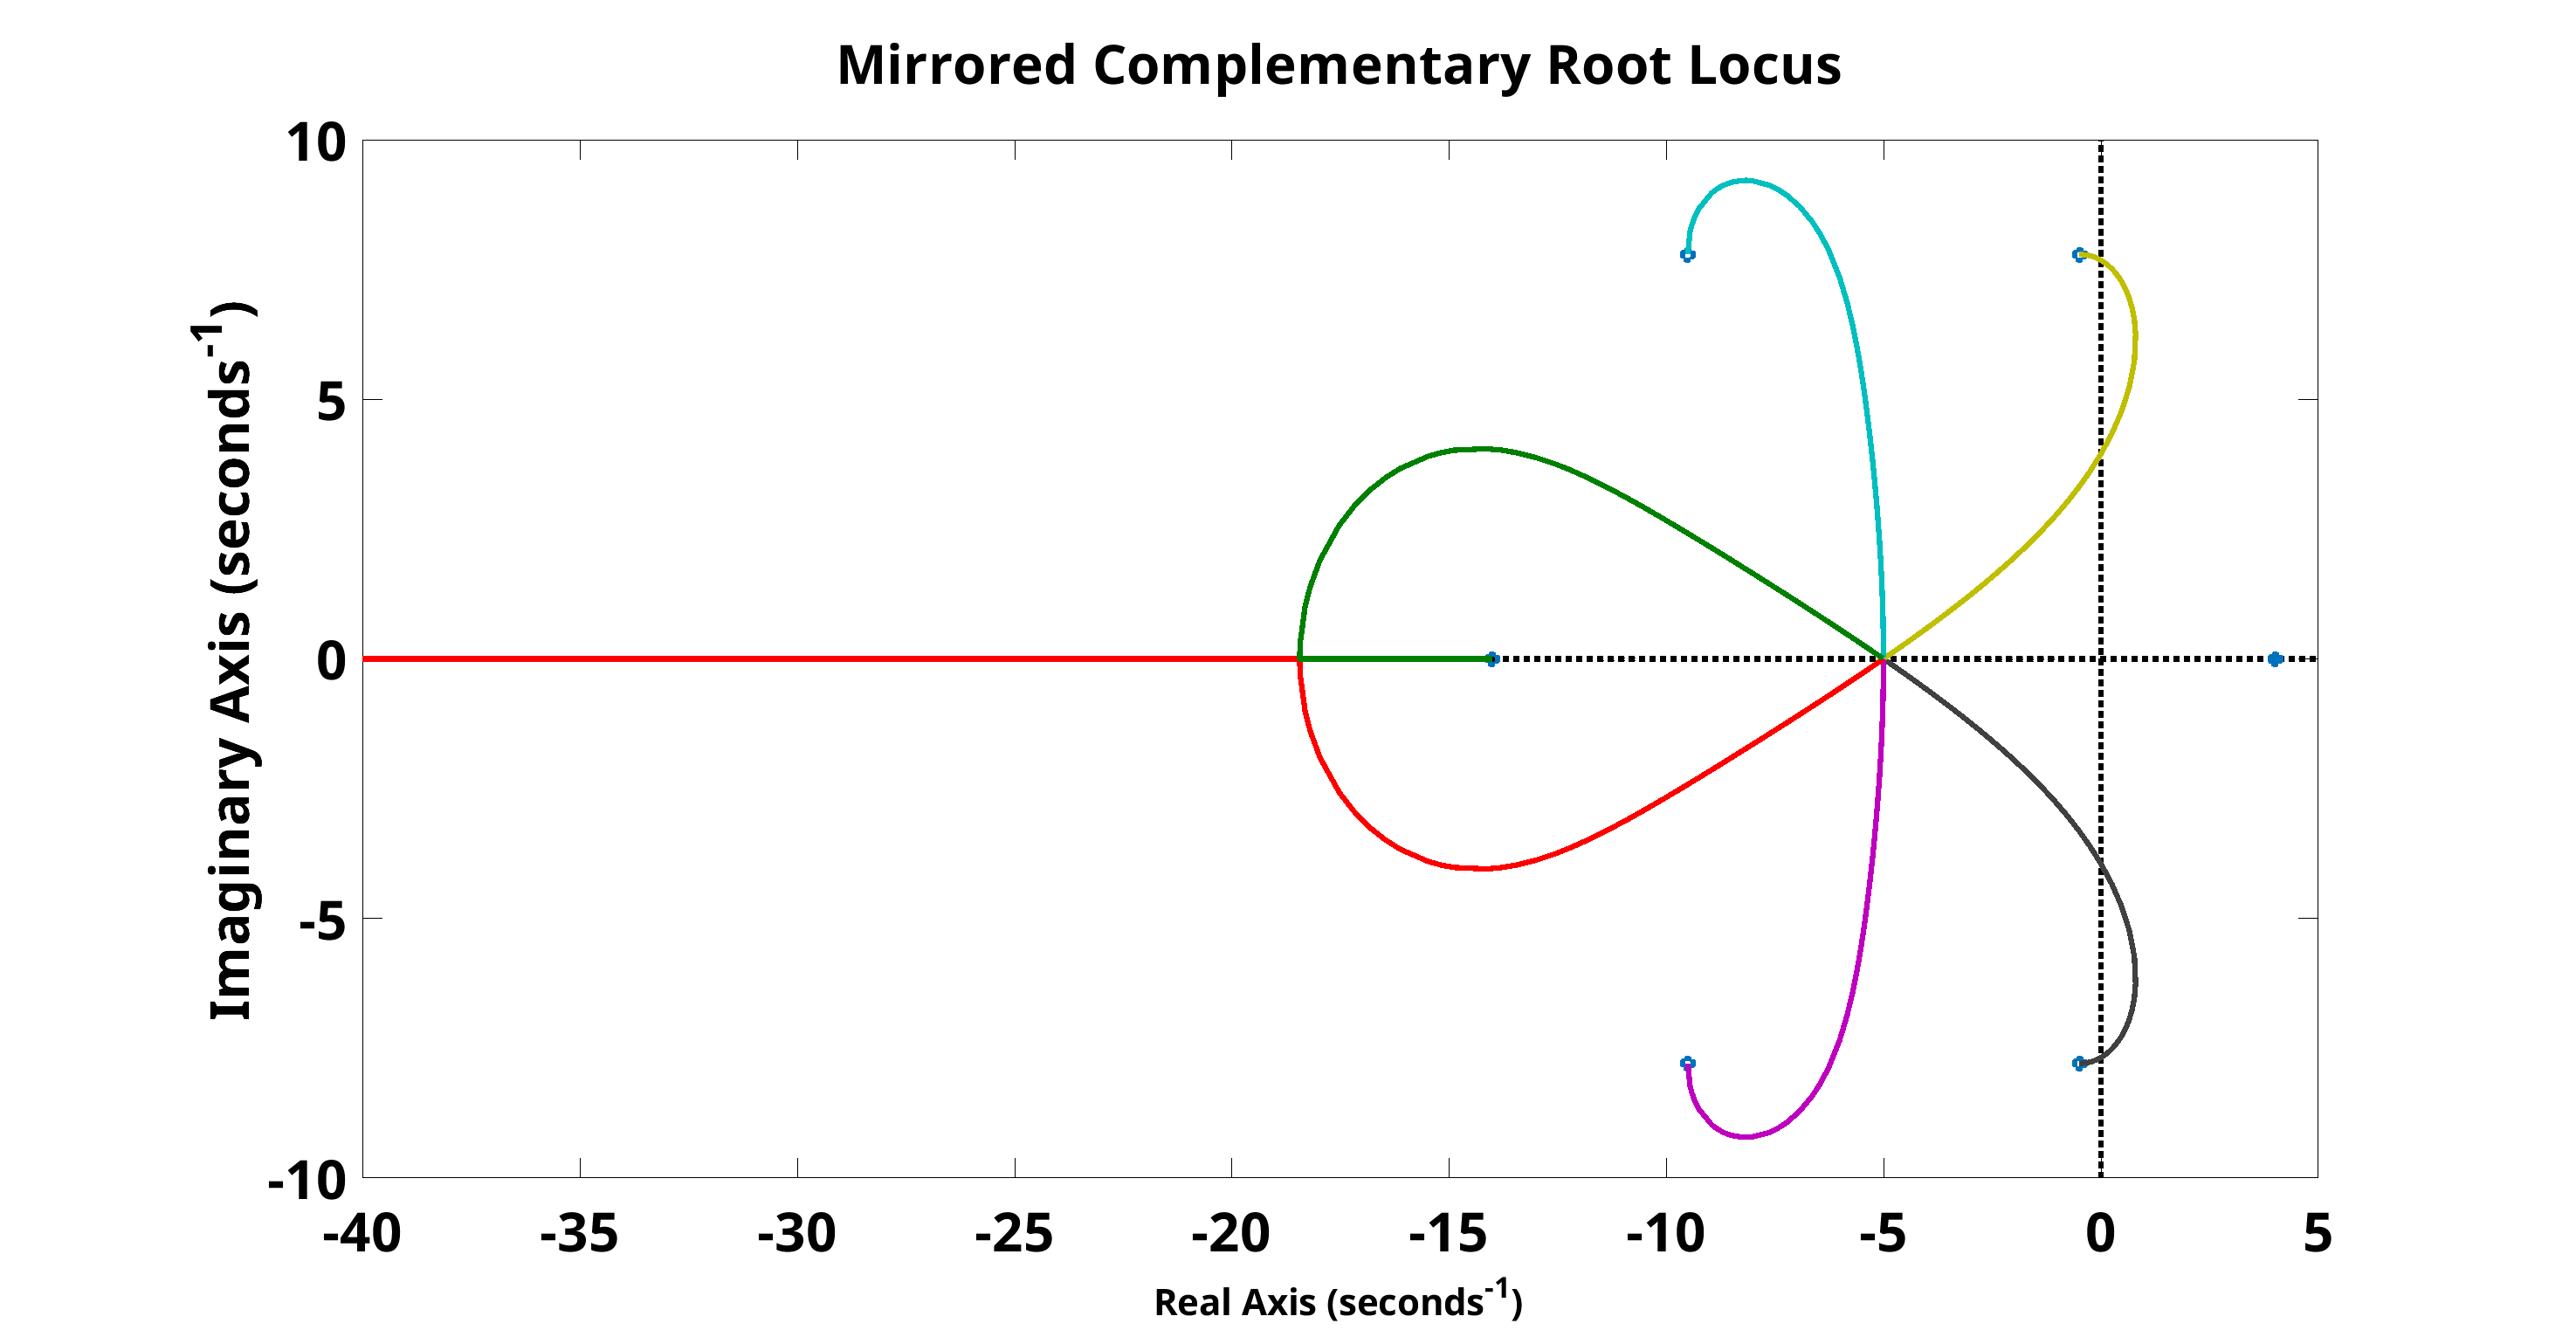
\includegraphics[width=\textwidth, keepaspectratio]{3_Images/NewMirroredCRLShiftedByInverseGammaSquarewithalpha9.eps}
		\caption{Shifted Root Locus bounded by $\mathfrak{Re}(s) = 4$.}
		\label{fig:MirroredComplimentaryRootLocus}
	\end{subfigure}
	\caption{Complementary root locus design for root-node loop ($x_1 = 1, \ell = 6$) under $\alpha = 9$.}
	\label{fig:RootLocus_plots}
\end{figure}

\begin{figure}[ht!]
	\centering
	\begin{subfigure}[b]{\textwidth}
		\centering
		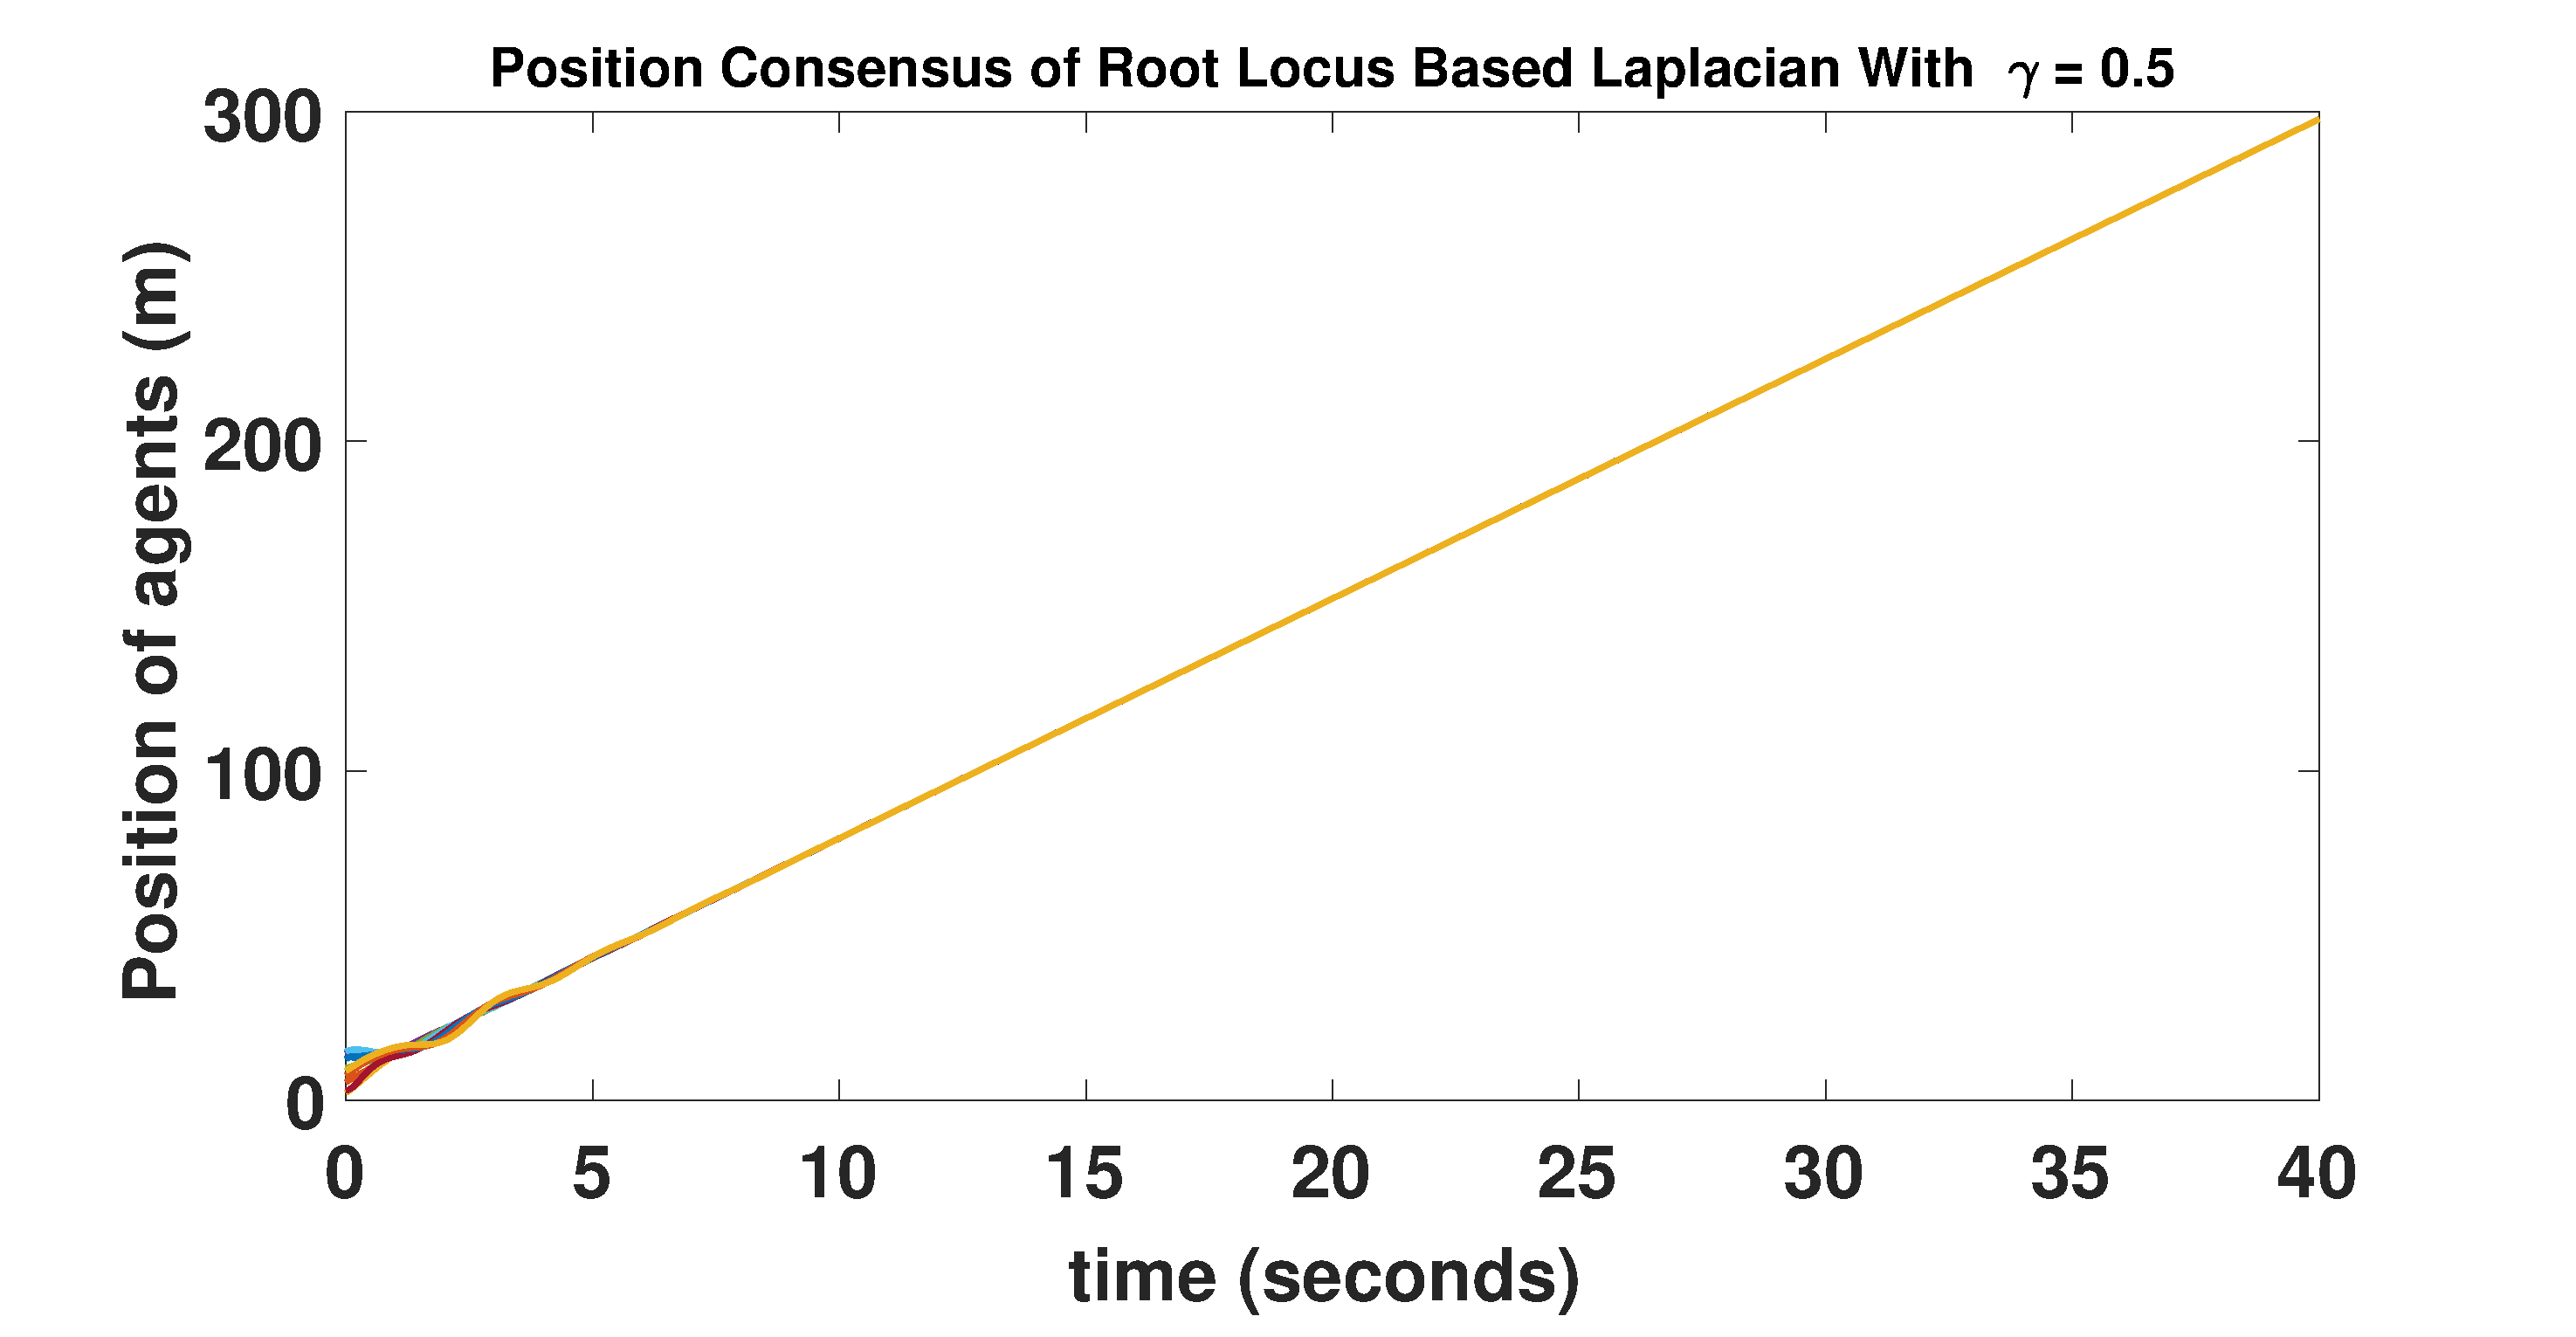
\includegraphics[width=\textwidth, keepaspectratio]{3_Images/NewRLBasedPositionConsensus0.5GammaBetaLessThanGM.eps}
		\caption{Root-Locus Position Consensus ($\gamma = 0.5$).}
		\label{fig:NewRootLocusBasedLaplacianPositionConsensus0.5}
	\end{subfigure}
	\hfill
	\begin{subfigure}[b]{\textwidth}
		\centering
		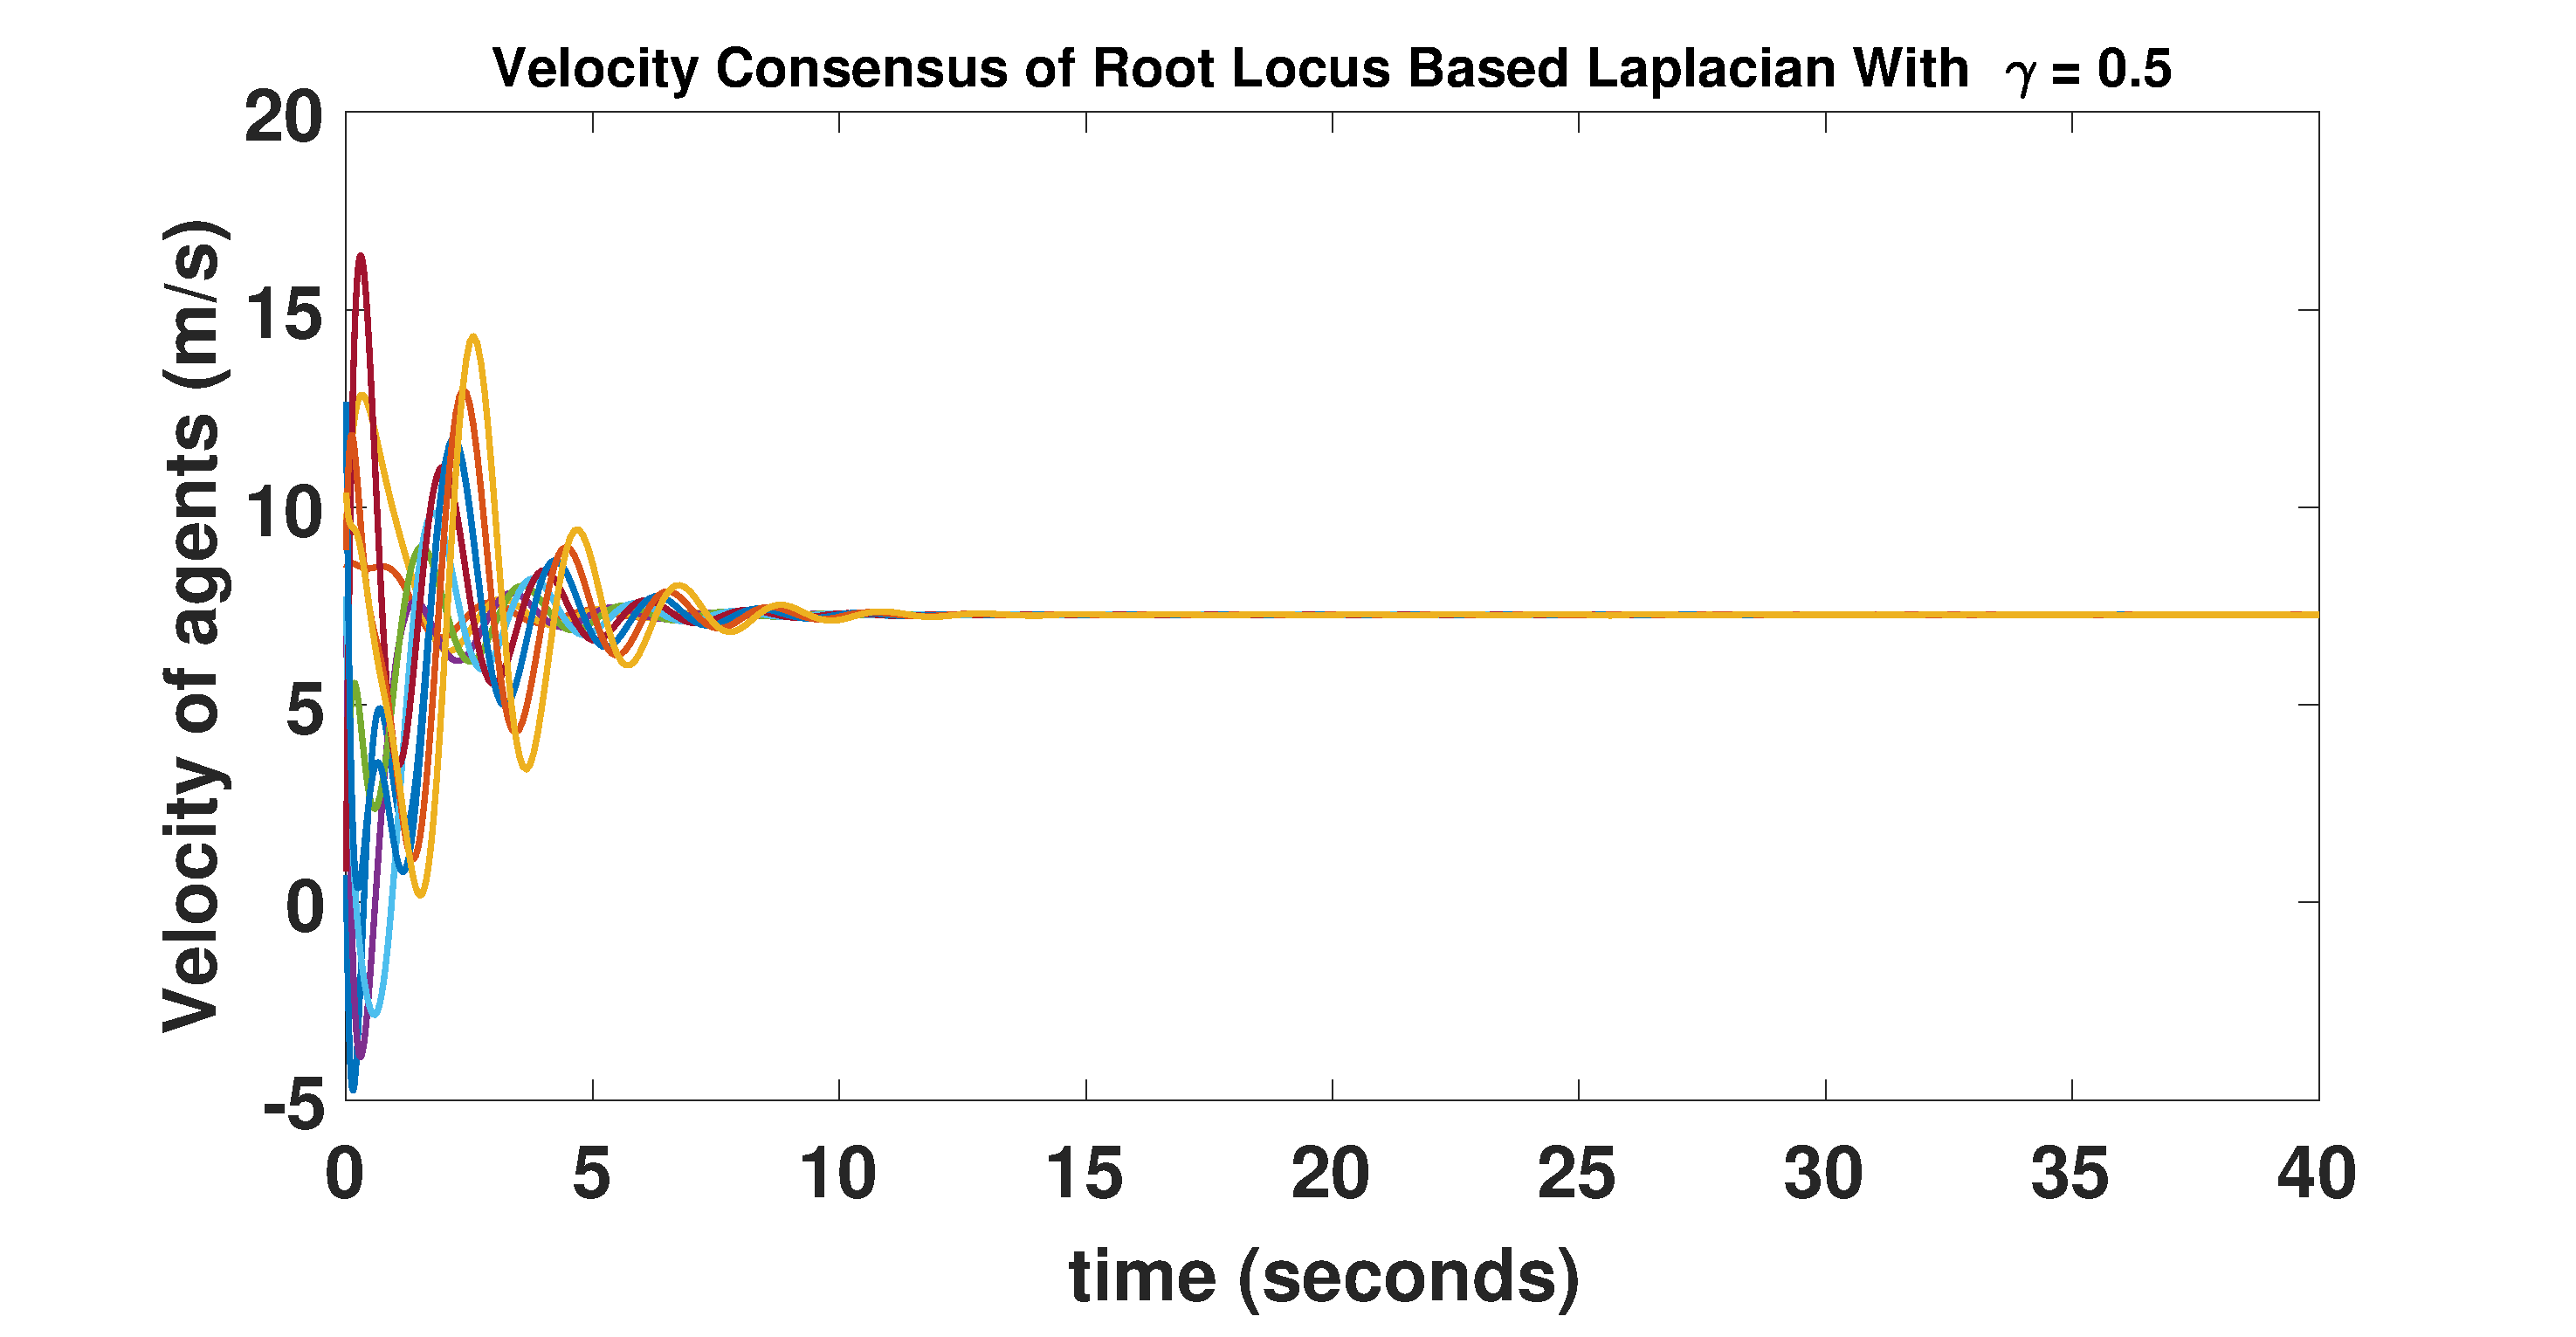
\includegraphics[width=\textwidth, keepaspectratio]{3_Images/NewRLBasedVelocityConsensus0.5GammaBetaLessThanGM.eps}
		\caption{Root-Locus Velocity Consensus ($\gamma = 0.5$).}
		\label{fig:NewRootLocusBasedLaplacianVelocityConsensus0.5}
	\end{subfigure}
	\caption{Position and velocity consensus restored for root-node loop ($x_1 = 1$) using Root-Locus design ($\alpha = 9, \beta = 0.6438$).}
	\label{fig:RootLocus_sims}
\end{figure}

\section{Summary}\label{sec:ch_GC_conclusion}

In this chapter, we presented a number of localized, decentralized control remedies to guarantee second-order consensus in directed chain networks subject to reverse feedback edges, resolving the theoretical limitations identified in Chapter \ref{ch:TwoReverseEdges}. The main contributions are:

\begin{itemize}
    \item \textbf{Gershgorin-Based Local Scaling (Leader-Exterior Loops):} For directed cycles where $x_1 > 1$, we formulated Node-Scaling, Edge-Scaling, and Combined-Scaling algorithms. By establishing that optimal disc separation occurs under an Arithmetic Progression (AP), we proved that tuning local factors to $p_1 \ge (\ell+1)/\gamma^2$ guarantees consensus under fixed global coupling parameters $\gamma$.
    \item \textbf{Root-Locus Remedy (Root-Node Loops):} For directed cycles involving Node 1 ($x_1 = 1$), where polynomial methods collapse, we formulated a complementary root-locus control framework, deriving exact upper bounds on gain $\beta$ that preserve stability.
    \item \textbf{Single-Gain Cyclic Pursuit Synthesis:} To eliminate edge-weakening, we derived a closed-form equal-weight threshold ($\alpha \ge \frac{\cot^2(\pi/(\ell+1))}{2\gamma^2}$) based on cyclic pursuit geometry, guaranteeing consensus without treating any loop edge indifferently.
\end{itemize}
\vspace{0.5em}
\noindent %\textbf{Transition to Chapter \ref{ch:Robustness_Analysis}:}\\
While Chapters \ref{ch:TwoReverseEdges} and \ref{ch:Guaranteed_Consensus} established exact deterministic stability boundaries and localized remedies for cyclic networks, real-world multi-agent systems operate under exogenous process noise and sensor measurement disturbances. 

To evaluate how directed cycles, spatial loop placement, and structural overlap dictate noise propagation and transient energy attenuation, Chapter \ref{ch:Robustness_Analysis} transitions from deterministic stability to systemic performance optimization, utilizing reduced-order edge dynamics ($\Sigma_e$) and suitable Lyapunov equations to derive closed-form expressions for the network $\mathcal{H}_2$ norm.
